\documentclass{article}
\usepackage{fontspec}
\usepackage{xcolor}
\usepackage{fancyhdr}
\usepackage[a4paper, margin=2.5cm]{geometry}
\usepackage{pdfpages}
\usepackage{titlesec}
\usepackage{indentfirst}
\usepackage{setspace}
\usepackage{tocloft}
\usepackage{graphicx}
\usepackage{amsmath}
\usepackage{amsfonts}
\usepackage{subfig}
\usepackage{cite}
\usepackage{appendix}

% Устанавливаем шрифты
\setmainfont{Calibri}
\setsansfont{Arial}
\definecolor{header_blue}{HTML}{2f5496}
\setcounter{secnumdepth}{4}

\renewcommand{\Huge}{\fontsize{36pt}{40pt}\selectfont}
\renewcommand{\normalsize}{\fontsize{11pt}{12pt}\selectfont}
\renewcommand{\Large}{\fontsize{13pt}{14pt}\selectfont}
\renewcommand{\huge}{\fontsize{18pt}{30pt}\selectfont}
\renewcommand{\LARGE}{\fontsize{16pt}{30pt}\selectfont}
\renewcommand{\large}{\fontsize{12pt}{13pt}\selectfont}

% Изменение шрифта
\renewcommand{\cftsecfont}{\normalfont} % Обычный шрифт для разделов

% Добавление точек между названием главы и номером страницы
\renewcommand{\cftsecleader}{\cftdotfill{\cftdotsep}} % Заполнение точками между названием главы и номером страницы

\renewcommand{\contentsname}{}
\renewcommand{\listfigurename}{}
\renewcommand{\cftfigpresnum}{Figure }
\setlength{\cftfignumwidth}{4.5em}
\renewcommand{\listtablename}{}


\titleformat{\section}
{\color{header_blue}\LARGE}{\thesection}{1em}{}
\titleformat{\subsection}
{\color{header_blue}\Large}{\thesubsection}{1em}{}
\titleformat{\subsubsection}
{\color{header_blue}\Large}{\thesubsubsection}{1em}{}

\titleformat{\subsubsubsection}[runin]{\normalfont\bfseries}{\thesubsubsubsection}{1em}{}
\titlespacing*{\subsubsubsection}{0pt}{3.25ex plus 1ex minus .2ex}{1em}

\begin{document}


\includepdf[pages=1]{title_page.pdf} % Title page
\newpage
\pagenumbering{roman}
\setcounter{page}{1}
\section*{Abstract}
\addcontentsline{toc}{section}{Abstract}
This report provides a description of the road marking recognition project.

The Duckietown project uses a light-sensitive road marking recognition algorithm as a baseline. It is fast and consistent in constant light conditions. However when 
the lightning changes (different weather, time or even just one broken lamp in the room) this algorithm should be adjusted by changing its config file. 
It is a pretty suboptimal solution, which makes developers of the Duckietown project rebuild their solutions each time the light conditions are changed. 
Assuming that the Duckietown project imitates real autonomous driving cars and the idea of the smart city, rebuilding the solution for autopilot because of the 
change of the daytime doesn't look like a good imitation of the real system. So it was decided to create a new algorithm for detecting road markups, based on a deep learning 
(DL) algorithm. This approach makes the algorithm light-independent.
The report describes in detail the mathematical foundations of the algorithms used in the project, as well as a description of the overall design and implementation. 
In addition, collecting and marking up the dataset for DL is described in this report.
As a result, the algorithm was created and the dataset was published. This algorithm was tested in Joint Advanced Student School (JASS) 2024 by JetBrains and was pretty 
successful.

\section*{Attestation}
\addcontentsline{toc}{section}{Attestation}
\noindent 
I understand the nature of plagiarism, and I am aware of the University’s policy on this.
\\
I certify that this document reports original work by me during my University project.

\vspace{1cm}

\noindent Signature: Ilia Nechaev

\vspace{1cm}

\noindent Date: 29.02.2024

\section*{Acknowledgements}
\addcontentsline{toc}{section}{Acknowledgements}
\setlength{\parskip}{10pt}
\noindent Special thanks to Mr.\ Konstantin Chaika for helping and guidance in Duckietown world.

\noindent Also I'd like to thank JetBrains for an opportunity to participate in JASS 2023, where I discovered Duckietown and decided to learn more about computer vision. 

\noindent It's also important to say thanks to UCLan Cyprus for providing me with the Duckiebot and Dr.\ Panayiotis Andreou for helping me with the paperwork.

\noindent Special thanks to my roommates: Ivan Iambarshev, Vasilii Telnov, Daria Chystiakova and Vadim Volkov for help in collecting the dataset and emotional support.

\noindent Also I'd like to say thanks to my teachers: Dr.\ Sergey Nikolenko, Dr.\ Vlad Shakhuro, Mr.\ Andrey Stotski, Mr.\ Anton Alexeev, Dr.\ Alexander Avdushenko
for giving an amazing start in machine learning and computer vision.

\noindent And of course a big thanks to my parents: Mrs.\ Natalia Nechaeva and Mr.\ Andrey Nechaev for support in any meaning of this word.

\section*{Table of Contents}
\addcontentsline{toc}{section}{Table of Contents}
\tableofcontents
\newpage

\section*{List of tables}
\addcontentsline{toc}{section}{List of tables}
\listoftables % Создание списка таблиц
\newpage

\section*{List of figures}
\addcontentsline{toc}{section}{List of figures}
\listoffigures % Создание списка рисунков
\newpage

\pagenumbering{arabic}
\setcounter{page}{1}

\section{Introduction}
\subsection{Background}

Thanks to the development of technology, self-driving cars and robots have become our daily routine, they have already changed and continue to change
the paradigms of transport and automation in various industries such as delivery, taxi, trucking and more.
The combination of the development of machine learning, robotics, mechatronics and input systems (cameras, lidars, radars, etc.) has become an important step towards
improving self-driving cars, robots and other systems, providing incredible opportunities and prospects in other areas.

Because of innovations in computer vision especially with using machine learning and deep learning as well as different types of sensors cars with autopilot and 
bots got a breakthrough in development.
Tesla with its autopilot for electric cars, Amazon with its research and implementation of autonomous delivery bots and other companies are great examples
of developing the industry.
These companies use different technologies like deep learning and different sensors (like lidars, cameras, gyroscopes, etc) for developing their algorithms.

The detection and labeling of environmental objects is an important factor for the operation of the perception system, which ensures the correct 
operation of autonomous cars and bots. To ensure safe and effective autonomous operation, detection and labeling processes must be configured accurately 
and reliably since these systems aim to simulate human perception and the ability to make their own decisions in unforeseen situations.

The perception and interpretation of complex environmental stimuli in real-time is made possible for autonomous vehicles and bots mainly through the use of 
detection and labeling algorithms. Using sensor data from cameras, lidar, radar and other detection tools, these algorithms simplify the search and identification 
of objects, obstacles and road infrastructure around the car. Also, accurate detection and labeling capabilities increase the vehicle's environmental awareness and 
allow proactive decisions to be made in dynamic driving conditions. Examples of how these algorithms work are the ability to distinguish between road signs,
road markups, as well as pedestrians and cyclists.

For the full functioning of a vehicle in autonomous driving scenarios, accurate identification and labeling of possible hazards is crucial to reduce risks 
and ensure the prevention of various types of accidents. Active collision avoidance techniques such as emergency braking or maneuverable steering are made 
possible by fast and well-established detection and marking systems that recognize and classify objects and obstacles in the path of an autonomous vehicle. 
Reliable detection algorithms also have the ability to predict unforeseen situations to some extent, such as unexpected pedestrian crossings or strange vehicle 
behavior, and respond to them with the slightest delay, increasing overall road safety and thus reducing the risk of accidents.

In addition to recognizing objects, labeling algorithms help with semantic understanding and contextual interpretation of the environment. 
These methods allow a vehicle to distinguish between different types of objects (for example, vehicles, pedestrians and bicycles) and draw conclusions about 
their possible behavior by providing semantic labels and attributes to identified elements and entities. Making rational navigation decisions, such as giving 
way to pedestrians at pedestrian crossings or reconciling complex traffic scenarios with numerous parallel interacting road users, depends on this semantic 
understanding.

Reliability, as well as the ability to adapt to rapidly changing circumstances, are also necessary for detection and marking systems to cope with their 
inherent unpredictability and variety of situations in the real world. Autonomous vehicles and robots face a number of obstacles and circumstances that 
affect the accuracy of detection and labeling algorithms, such as changing lighting conditions, interference or noise in sensors. Therefore, in order to improve 
the performance of these algorithms and generalization capabilities in various work situations, continuous optimization and refinement using machine learning and 
methodologies based on the data obtained is crucial.

Summing up, we can say that the perception systems in autonomous cars and bots mostly rely on detection and labeling systems as fundamental building blocks that 
allow them to perceive, see, understand and overcome difficult situations on their own. In order to ensure safer and more efficient autonomous operation, 
and in addition to increase awareness of the autonomous transport environment, as well as reduce risks and facilitate smooth interaction with it, detection and 
labeling algorithms must be sufficiently accurate, reliable and flexible.

\subsection{Context}
In March \- April of 2023 I was a participant in Joint Advanced Student School (JASS) by JetBrains. 
There we developed a smart city prototype using the Duckietown project. I have noticed that Duckiebots \- robots that imitate self-driving cars in a smart city behave 
differently with different lightning. For example, we always kept curtains closed, but if the wind flow opened them the bot started driving unpredictably.

After a small investigation, I've discovered, that the current algorithm that is run on Duckiebots is based on segmenting pixels by colors. This approach is good when 
light conditions are constant, but each time they change (new room with different lightning or changing time in a room with opened curtains) 
the bot needs recalibration. Also important to mention that each Duckiebot has LED lights that can be almost any color which can lead to wrong detection.

\begin{figure}[htbp]
    \centering
    \subfloat[Raw image of the road with the first light condition]{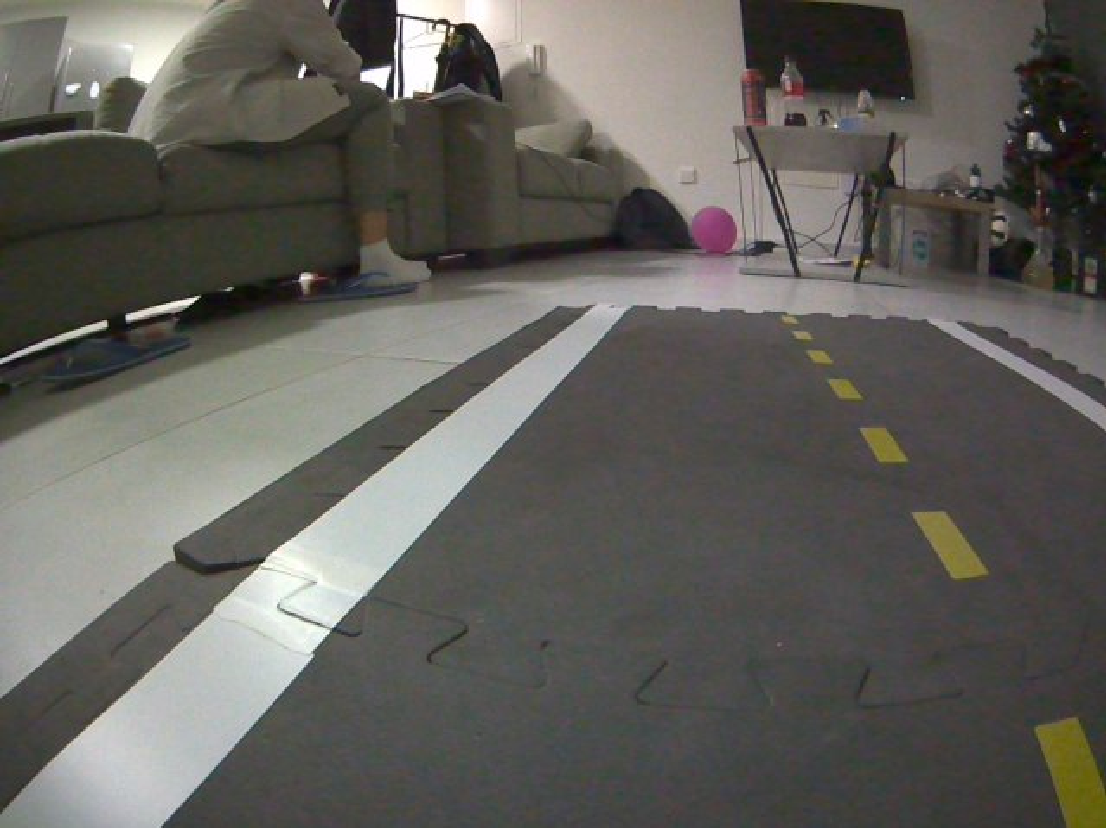
\includegraphics[scale=0.1]{src/Introduction/assets/old_masks2.png}}
    \subfloat[Mask of the road with the first light condition]{
\includegraphics[scale=0.1]{src/Introduction/assets/old_masks1.png}}
    \\
    \subfloat[Raw image of the road with the second light condition]{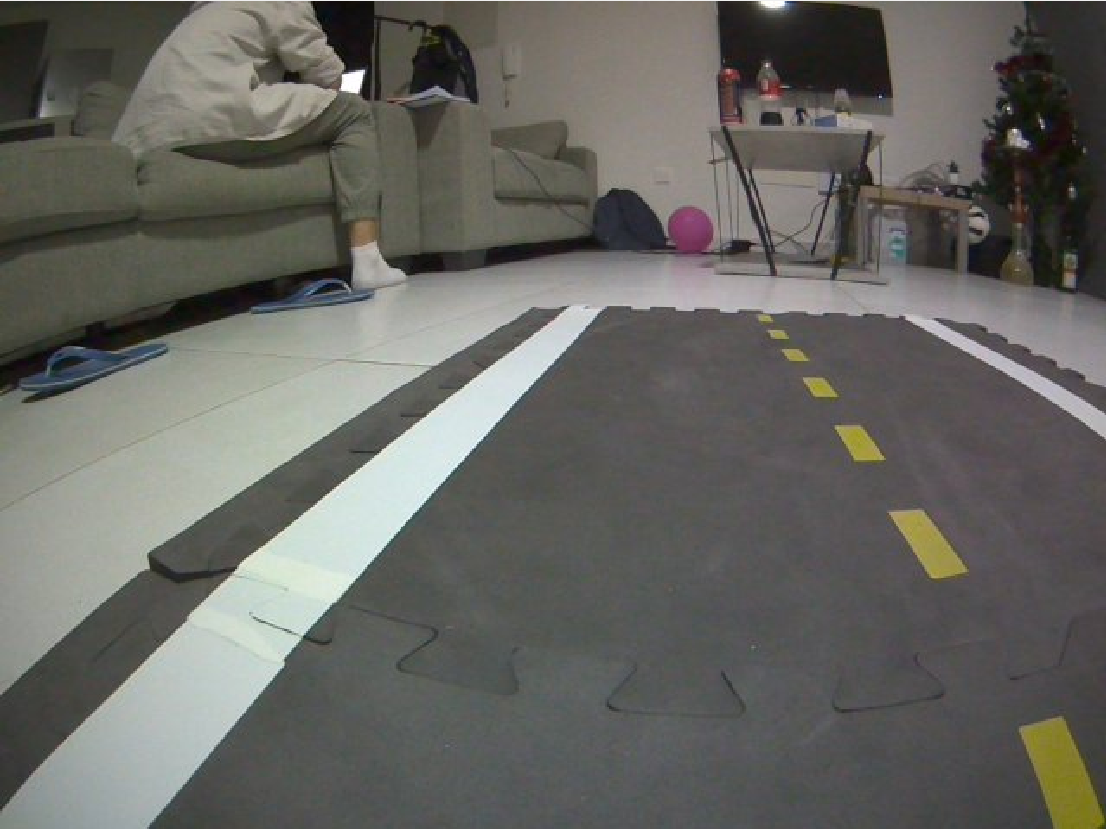
\includegraphics[scale=0.1]{src/Introduction/assets/old_masks3.png}}
    \subfloat[Mask of the road with the second light condition]{
\includegraphics[scale=0.1]{src/Introduction/assets/old_masks4.png}}
    \caption{Old algorithm segmentation with different light conditions}\label{fig:old_masks}
\end{figure}
\subsection{Applicability of Findings to the Commercial World}

So after this observation, the idea of developing a light-insensitive road markup detection algorithm came to my mind. 
I wanted to create an algorithm based on the deep learning (DL) approach, so it would be easy to scale (in terms of developing a new neural network), 
light-insensitive, but at the same time light in computational terms.


\subsection{Bot specification}
The idea of using the DL approach came to me as soon as 
I've discovered that Duckiebots can be powered by Jetson Nano by Nvidia.

\begin{table}[h]
    \centering 
    \begin{tabular}{|c|c|}
        \hline
        AI Performance & 472 GFLOPs \\ \hline
        GPU & 128-core NVIDIA Maxwell™ GPU \\ 	\hline
        CPU & Quad-Core ARM® Cortex®-A57 MPCore  \\ \hline
        Memory & 4GB 64-bit LPDDR4 Memory \\ \hline
        Storage & Micro SD \\\hline
    \end{tabular} % Конец определения столбцов таблицы
    \caption{Jetson nano specs} % Подпись к таблице
    \label{tab:example} % Метка для ссылки на таблицу
\end{table} % Конец окружения таблицы

4GB of RAM and 128 CUDA cores are more than enough for a lightweight 
convolutional neural network (CNN)
\section{Background reading}
\subsection{Introduction}
Creating the algorithm for lane detection involves two major steps: collecting and marking
data and creating the algorithm itself. 

Lack of finance makes me find a way to mark up the dataset in an autonomous way. To do this
I will try non-ML and some unsupervised learning methods of marking.
The second step is creating the algorithm itself. After the CNN revolution that 
happened in CV more than 10 years ago, when AlexNet was presented\cite{alexnet}, many different approaches and
architectures were created, most of which can be used almost on any hardware for almost any task. 
In this review, my goal is to choose a few of them, test and find one that suits my task best.

\subsection{Data preprocessing}
\subsubsection{Introduction}
All ML projects start with collecting a dataset. So I followed the same procedure. 

The dataset was collected using Duckiebot. A small server was created 
using GoLang to receive images from the bot's camera. After that a few 
different approaches were used to mark it up. All approaches had some disadvantages that will
be listed below:

\subsubsection{Non-ML approach}
\begin{figure}[h]
    \begin{center}
        
    
    \subfloat[raw image]{\label{fig:lena-raw}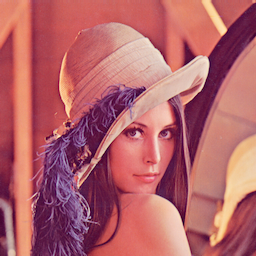
\includegraphics[scale=0.32]{src/BackgroundReading/assets/Lenna.png}}
    \subfloat[brightness map]{\label{fig:lena-brightness}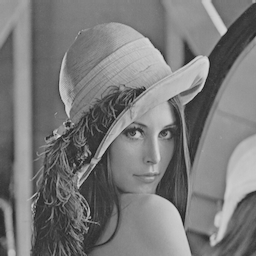
\includegraphics[scale=0.32]{src/BackgroundReading/assets/Lenna brightness.png}}
    \subfloat[energy map]{\label{fig:lena-energy}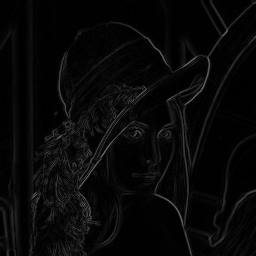
\includegraphics[scale=0.32]{src/BackgroundReading/assets/Lenna energy.png} }
    \subfloat[scaled energy map]{\label{fig:lena-scaled-energy}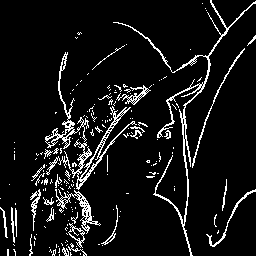
\includegraphics[scale=0.32]{src/BackgroundReading/assets/Lenna energy_with contrast.png}}
    \\
    \subfloat[raw image]{\label{fig:road-raw}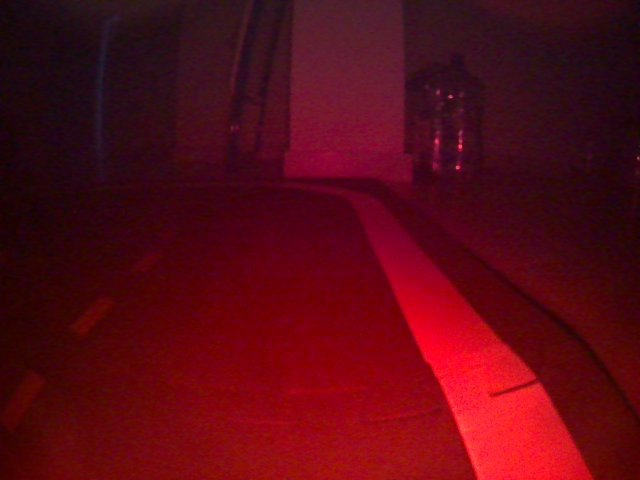
\includegraphics[scale=0.1295]{src/BackgroundReading/assets/615.png}}
    \subfloat[brightness map]{\label{fig:road-brightness}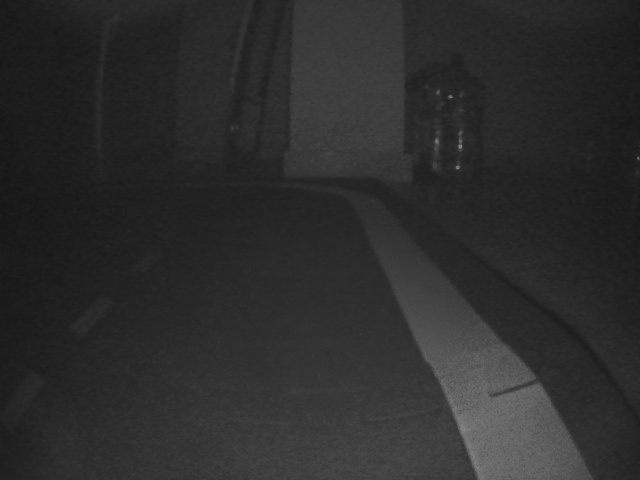
\includegraphics[scale=0.1295]{src/BackgroundReading/assets/615 brightness.png}}
    \subfloat[energy map]{\label{fig:road-energy}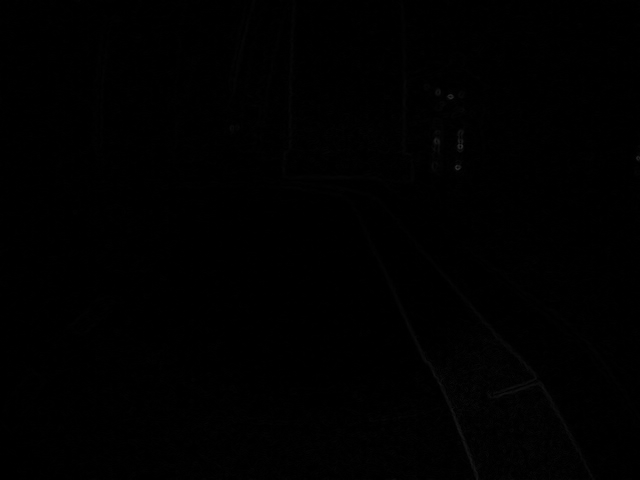
\includegraphics[scale=0.1295]{src/BackgroundReading/assets/615 energy.png} }
    \subfloat[scaled energy map]{\label{fig:road-scaled-energy}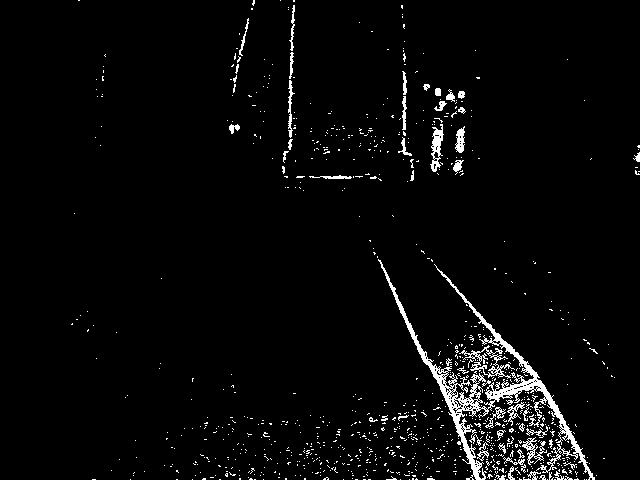
\includegraphics[scale=0.1295]{src/BackgroundReading/assets/615 energy_with contrast.png}}
    \end{center}

    \caption{Results of each step for high contrast and low contrast image}
\end{figure}
The first idea was to use a non-ML approach based on ``energy``.~\cite{seamcarving} 

The main ideas of this approach are:
\begin{enumerate}
    \item Convert RGB pixels to brightness
    \item Use discrete derivatives of brightness to compute energy
\end{enumerate}
\begin{enumerate}
    \item \textbf{Brightness}\\
To convert RGB image to brightness map it was decided to use Y 
component of YCbCr color space, because this component shows the 
brightness. To convert RGB image to YCbCr we need to use simple 
operation~\cite{YCbCr}:
\[\begin{pmatrix}
    Y' \\
    Cb \\
    Cr
\end{pmatrix} = 
\begin{pmatrix}
    0.257 & 0.504 & 0.098 \\
    -0.148 & -0.291 & 0.439 \\
    0.439 & -0.368 & -0.071
\end{pmatrix} \cdot
\begin{pmatrix}
    R \\
    G \\
    B
\end{pmatrix} + 
\begin{pmatrix}
    16 \\
    128 \\
    128
\end{pmatrix}\]
\item \textbf{Energy}
For energy, it was decided to use the formula from 
seam carving paper~\cite{seamcarving}:
\[e_1(I) = |\frac{\partial}{\partial x} I| + |\frac{\partial}{\partial y} I|\]
Where 
\[|\frac{\partial}{\partial x} I_{i,j}| = \frac{I_{i+1,j} - I_{i-1,j}}{2}\]

The intention was to use this algorithm to find a contour of road markup. 
Unfortunately, this approach performs well on high-contrast images, but the project's problem is that images in the dataset 
can and should be low contrast. So this method was abandoned.
\end{enumerate}

\subsubsection{KNN approach}
\begin{figure}[h]
    \begin{center}
    \subfloat[Raw image]{\label{fig:edge-a}
\includegraphics[scale=0.2]{src/BackgroundReading/assets/Raw.png}}
    \subfloat[Middle lane mask]{\label{fig:edge-b}
\includegraphics[scale=0.2]{src/BackgroundReading/assets/Middle line.png}}
    \subfloat[Side lane mask]{\label{fig:edge-c}
\includegraphics[scale=0.2]{src/BackgroundReading/assets/Side line.png} }
    \subfloat[Road mask]{\label{fig:edge-d}
\includegraphics[scale=0.2]{src/BackgroundReading/assets/Road.png}}
    \end{center}
    \caption{Masks provided by KNN algorithm}
\end{figure}
The second thought was about KNN~\cite{knn}. It's powerful, but the computational heavy clustering algorithm can be used in unsupervised learning. 
I tried to use it in two ways:
\begin{enumerate}
    \item Use only color for clustering
    \item Use colors and position of pixels
\end{enumerate}

Both approaches had their advantages and disadvantages, but in the end this method
was rejected, because it couldn't provide good markup even on 
bright images.

\subsubsection{EM algorithm}
\begin{figure}[h]
    \begin{center}
        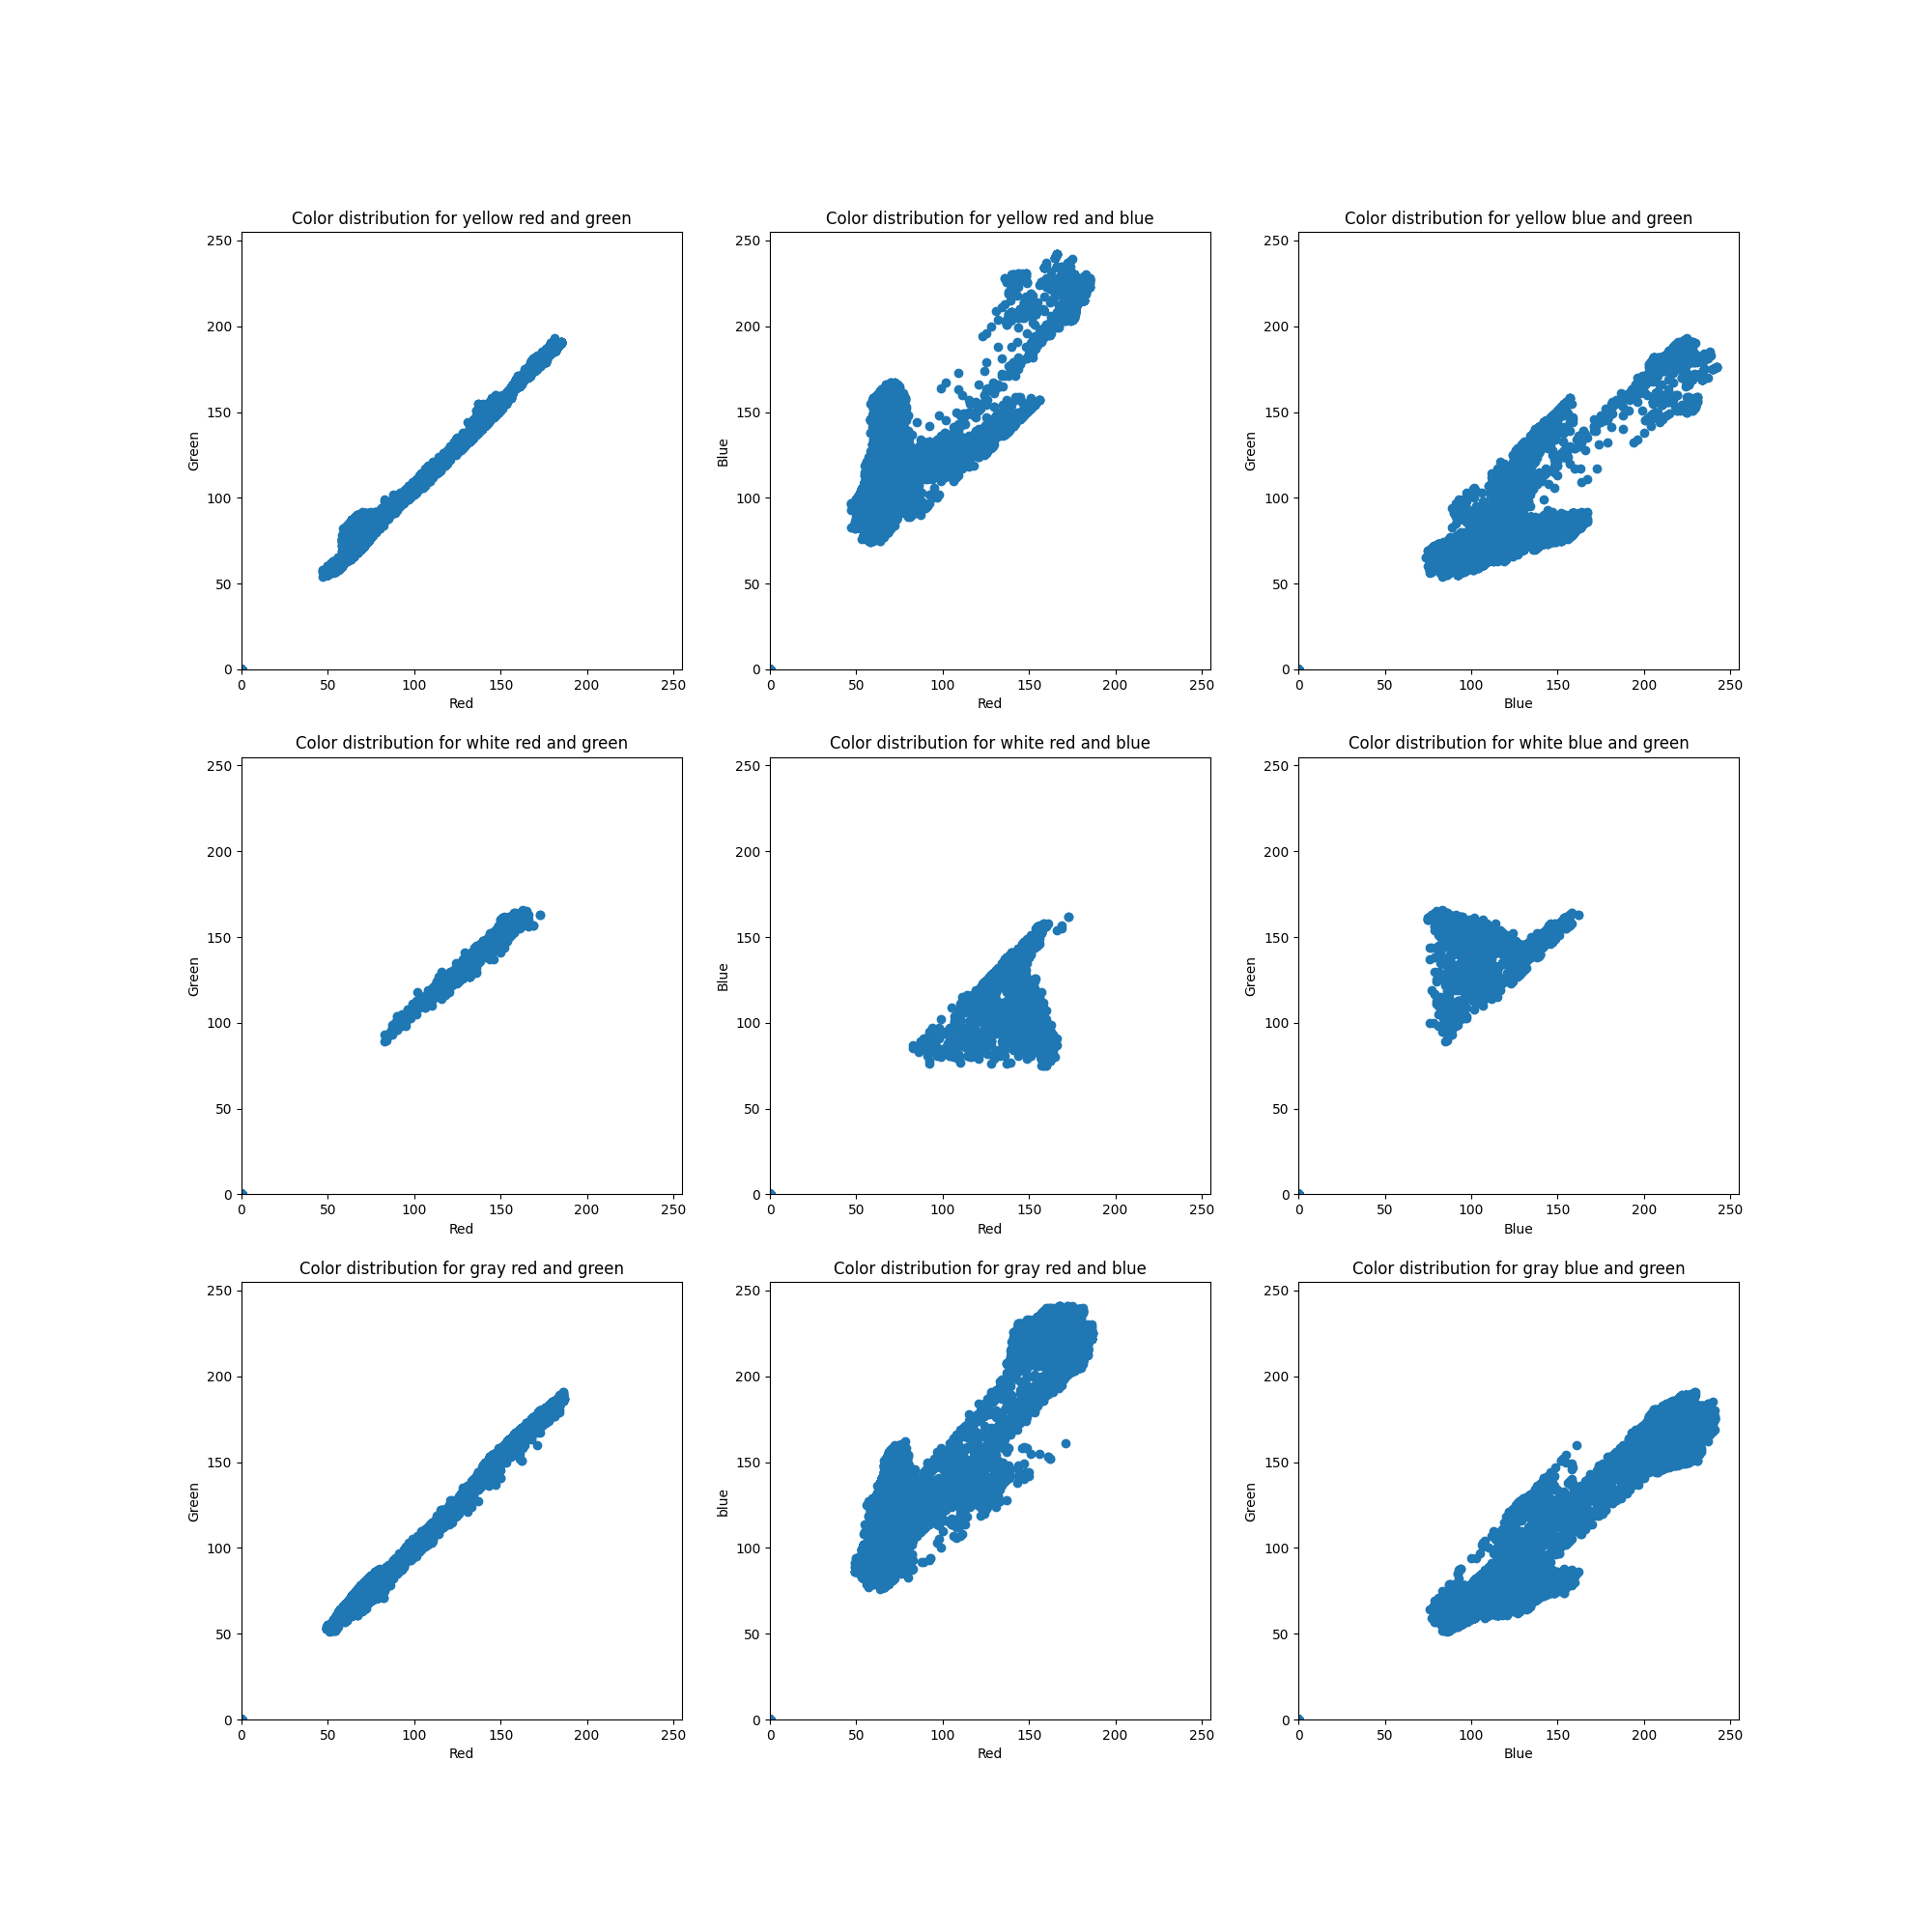
\includegraphics[scale=0.232]{src/BackgroundReading/assets/Distr.png}
    \end{center}
    \caption{Color distribution on images}
\end{figure}

\begin{figure}[h]
    \begin{center}
    \subfloat[Raw image bad sample]{\label{fig:road-raw-bad}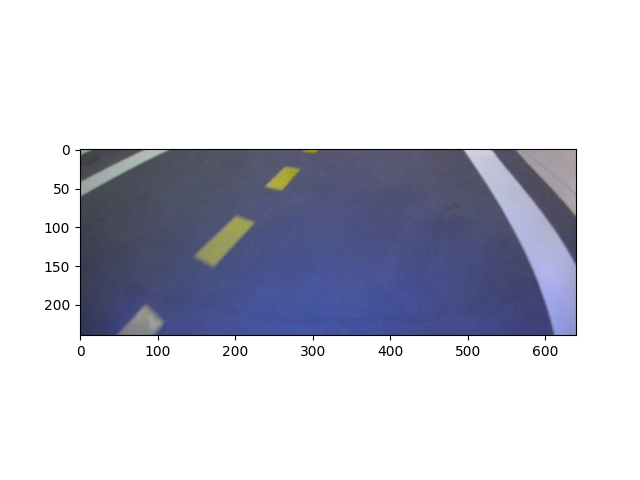
\includegraphics[scale=0.17]{src/BackgroundReading/assets/RawEMBad.png}}
    \subfloat[Mask bad sample]{\label{fig:road-mask-bad}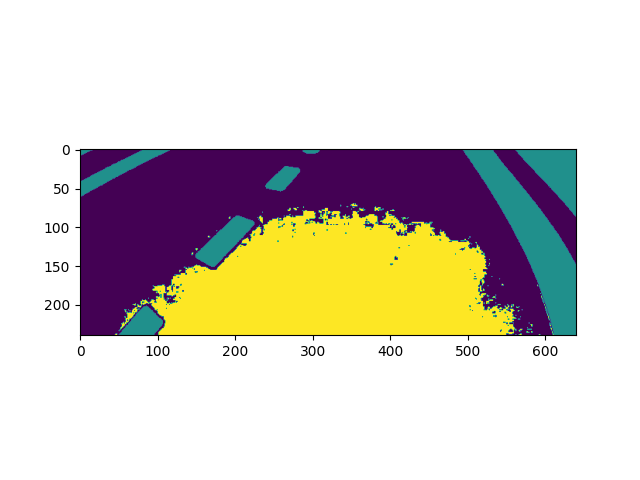
\includegraphics[scale=0.17]{src/BackgroundReading/assets/MaskEMBad.png}}
    \subfloat[Raw image good sample]{\label{fig:road-raw-good}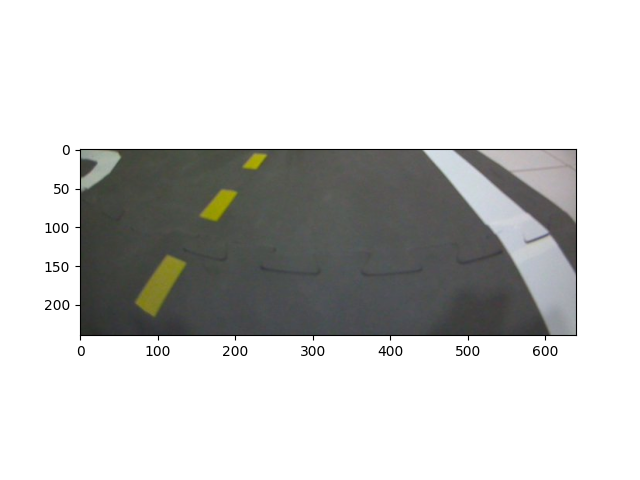
\includegraphics[scale=0.17]{src/BackgroundReading/assets/RawEMGood.png} }
    \subfloat[Mask good sample]{\label{fig:road-mask-good}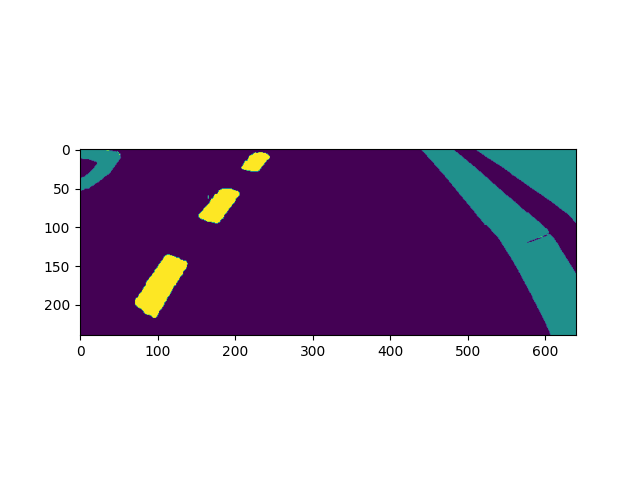
\includegraphics[scale=0.17]{src/BackgroundReading/assets/MaskEMGood.png}}
    \end{center}
    \caption{Masks provided by EM algorithm}
\end{figure}


Last hope was the EM\cite{em1}\cite{em_algo_2} algorithm. The idea of the EM algorithm is to use 
general knowledge about our world to predict something. In my case, I assumed 
that the color distribution of each image is a mixing of a few Gaussians. 

Assumptions:
\begin{enumerate}
    \item Colour distribution is formed by three Gaussians with parameters: 
    \\
    $\{\bar\mu_1, \Sigma_1\}, \{\bar\mu_2, \Sigma_2\}, \{\bar\mu_3, \Sigma_3\}$
    \item Choosing gaussian is made with probabilities: $\{\pi_1, \pi_2, \pi_3\}$
\end{enumerate}

PDF of Normal distribution is
    
    \[\mathcal{N}(\bar x | \mu, \sigma) = \displaystyle \frac{1}{\sigma \sqrt{2\pi}} \cdot e^{\displaystyle-\frac{1}{2}{(\frac{x-\mu}{\sigma})}^2}\]


The idea of the EM algorithm is simple:
\begin{enumerate}
    \item E-step: fix $\bar\theta$ \- parameters of model, find $\mathbb{E}[z]$ \- math expectation of hidden parameters:

    \[\mathbb{E}[z_{n, k}] = \displaystyle \frac{\pi_k\cdot \mathcal{N}(\bar x_n | \bar \mu_k, \Sigma_k)}{\sum\limits_{l=1}^K \pi_l \cdot \mathcal{N}(\bar x_n | \bar \mu_l, \Sigma_l)}\]
    \item M-step: fix $\mathbb{E}$ and maximize likelihood: $\mathbb{E}[\log p(x,z|\bar\theta)] \overset{}{\underset{\bar \theta}{\longrightarrow}} \text{max}$:

    \[\mathbb{E}[\log p(x,z|\bar\theta)] = \sum\limits_k\Big(\sum\limits_n\mathbb{E}[z_{n,k}]\Big) \log \pi_k + \sum\limits_k\sum\limits_n\mathbb{E}[z_{n,k}]\cdot \log p(\bar x_n|\bar\mu_k,\Sigma_k)\]

Also we can notice, that $\sum\limits_n\mathbb{E}[z_{n,k}] = \mathbb{E}[|C_k|]$, where $|C_k|$ is the amount of samples in cluster $C_k$
\end{enumerate}

The results of the EM algorithm were also poor, but a bit better than KNN's ones:

\subsubsection{Result approach}
The final approach is combining energy with EM, 
then using its outputs as inputs to logistic regression\cite{log_regression} with 
data augmentations\cite{augmentations}\cite{synthetic_data}. 

It was decided that this approach should be more useful, because:
\begin{enumerate}
    \item Data augmentations can help with the inefficient of previous approaches, 
    because applying color filters to `clean' images can emulate the light of LEDs 
    of the Duckiebot without loss of accuracy of EM algorithm predictions
    \item The noise of the labels can be compensated by the size of the 
    dataset\cite{big_data_less_noice}
\end{enumerate}

\subsection{Algorithm implementation}
\subsubsection{Introduction}
To implement the algorithm some DL approach will be used. 
There are a few ways to do it:
\begin{itemize}
    \item Fully connected NN to classify the color of pixel\cite{fully_connected} 
    \item MobileNet\cite{mobileNet}
    \item ShuffleNet\cite{shufflenet}
    \item EfficientNet\cite{efficientnet}
    \item Squeeze-and-Excitation Networks\cite{seNet}
\end{itemize}
\subsubsection{Fully connected NN}
This approach will be used as the baseline in terms of accuracy and computational 
speed

This architecture is extremely easy to implement and it is relatively fast.
~\cite{fully_connected} 
The key idea of fully connected NN is MLP (multi-layer perceptron):

If we have input tensor $X\in \mathbb{R}^{n\times 1}$, we can apply linear transformation to it:
$W\cdot X$, where $W \in \mathbb{R}^{k\times n}$, after that we need to add some 
nonlinear activation (ReLU, sigmoid, Tanh, etc) and apply the same block a few more times
As the last activation, we can use softmax for classification or just leave it as it is for regression

\begin{figure}[ht]
    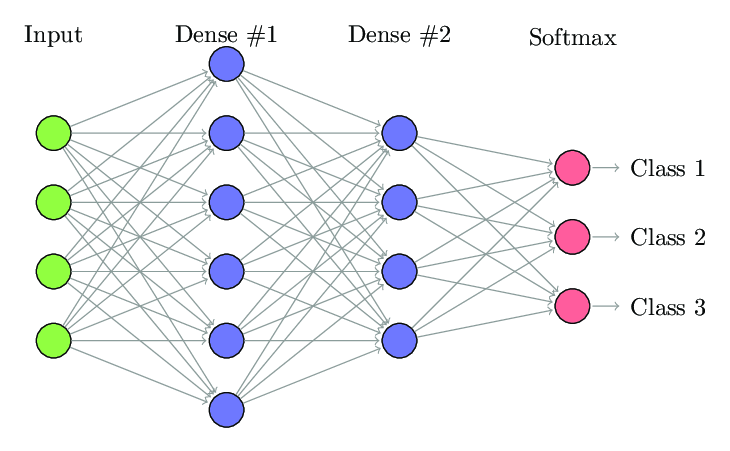
\includegraphics[scale=0.5]{src/BackgroundReading/assets/fully_connected.png}
    \caption{Architecture of fully connected NN with 3 layers}
\end{figure}


But this type of NN isn't so popular in computer vision, because it can't handle 
random-sized images without preprocessing and it struggles with detecting objects 
in different parts of the image. But in the case of this task, it will not be a problem, 
because all images will be the same shape and objects will be in approximately the same spots.
However using a hole image as input tensor will be tough because the image size is $320\times480$ pixels,
so the input tensor will be of size 153600, even if a relatively small hidden layer is used (10000 neurons), 
then one forward pass will be about 23,5 GFLOPs, which is much bigger than CNNs consume.
So this architecture can be used to determine the color of each pixel only independently from others,
this will affect accuracy because such an approach can't determine objects, only colors, which is
good as a baseline, but can't be used in production. 

Determining pixel color will require an input tensor of size 3 (or 5 if positional embeddings are used), 
output tensor will be of size 3 (to show probabilities of belonging pixel to yellow, white or gray color)
and hidden layer can be any size because as a result flops will be: $153600 \cdot( 3 \cdot n + n \cdot 3) = 921600 \cdot n$ FLOPs
if $n$ is less than 20, then such NN can't use more than 18 MFLOPs which is good in comparison with CNN

\subsubsection{MobileNet}
MobileNet Architecture family seems to be a more suitable approach 
as it is relatively fast and has pretty good accuracy on the ImageNet dataset.

Core idea of MobileNet\cite{mobileNet} is splitting standard convolution~\cite{cnn} on two steps:
\begin{itemize}
    \item Using convolution with one channel for each input channel (depthwise convolution)
    \item Use the result of the previous step as input for pointwise convolution 
    (convolution with $1\times 1 \times M$ kernel, where $M$ is amount of input channels) 
    \- this step lets us extract features
\end{itemize}
This approach is fast, because in usual convolution with kernel $D_K\times D_k\times M \times N$ 
(where $D_K$ is kernel size, $M$ \- amount of input channels and $K$ \- amount of output
channels) we need $D_K\cdot D_k\cdot M \cdot N \cdot D_F \cdot D_F$ operations per image 
(we can assume that all images are squared, it is the usual approach in CV). On the other hand in 
MobileNet architecture convolution needs only $D_F\cdot D_F \cdot M \big(D_K \cdot D_K + N)$ 
operations, so we have improved in 
\[ \frac{1}{\frac{1}{N} + \frac{1}{D_K^2}}\] 
Assuming that the usual kernel has size $3\times 3$ it is a significant boost.

Also, this approach reduces memory usage, because each convolutional layer needs
only $M \cdot D_K\cdot D_K + N\cdot M$ parameters, while classical convolutional layer
with the same input hyperparameters needs $M \cdot D_K\cdot D_K \cdot N$

\subsubsection{ShuffleNet}

This model develops ideas of MobileNet (even if it is not fully represented in paper, however, it's obvious).

Authors of ShuffleNet propose to use group pointwise convolution (GPC) instead of 
classical pointwise convolution\cite{shufflenet}. 

The idea of GPC is relatively simple: instead of performing this operation:
$I * K$ (where $*$ is convolution, $I$ is tensor with shape $H\times W \times C \times M$ 
and $K$ pointwise convolution kernel with shape $1\times 1 \times C \times M$, 
$C$ \- amount of input channels, $M$ \- amount of output channels), which
takes $W\cdot H \cdot C \cdot M$ MFLOPs (floating point multiplication-adds), we 
can use this operation:
\[\overset{g-1}{\underset{i=0}{CONCAT}}(I_{[i\cdot g : (i+1)\cdot g]}* K_i)\] 
where $I_{[a:b]}$ \- tnesor which consists of $a$'th till $b$'th channels of tensor $I$. 
Such an approach requires in $g$ times fewer MFLOPs, but we have to face another problem:
output channels, which were produced by one group of input channels `do not know' anything about 
other input channels. To fix this authors of ShuffleNet propose a shuffle layer, which
can be used in the bottleneck block (Figure~\ref{ShuffleNet architecture}).
\begin{figure*}[ht]
    \begin{center}
        \subfloat[ShuffleNet Bottleneck block]{\label{fig:bottle-neck}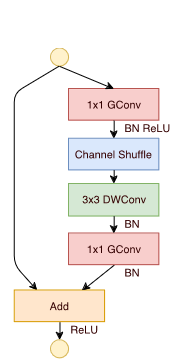
\includegraphics[scale=0.5]{src/BackgroundReading/assets/bottleneck.png}}
        \subfloat[Shuffle layer]{\label{fig:shuffle_layer}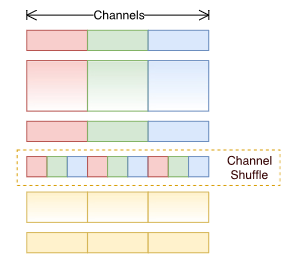
\includegraphics[scale=0.5]{src/BackgroundReading/assets/shuffle_layer.png}}
    \end{center}
    \caption{ShuffleNet architecture}\label{ShuffleNet architecture}
\end{figure*}

If we count MFLOPs of bottleneck block in ShuffleNet and MobileNet 
(we can use its ideas to construct bottleneck block), we will get such results:
\begin{enumerate}
    \item ShuffleNet: $W\cdot H \cdot (\frac{2\cdot C \cdot M}{g} + 9M)$
    \item MobileNet: $W\cdot H \cdot (2 \cdot C \cdot M + 9M)$
\end{enumerate}
As you can see we have a small gain, but we lose some accuracy, even in the article authors
provide us with data, that shows that ShuffleNet isn't always better than MobileNet,
so I will try to implement both of them to find the best one.

\subsubsection{EfficientNet}
EfficientNet also seems to be a good model to try\cite{efficientnet}. 

It uses MobileNetV2\cite{mobile_netv2} bottleneck as main building blocks and this type of architecture
is easy to scale. Moreover base model EfficientNet-B0 has fewer MFLOPs in comparison 
with MobileNet (390 MFLOPs vs 569 MFLOPs), but has a bit more parameters. However, 
the Duckiebot has 4GB RAM so it can handle up to 1 billion parameters, which is much 
bigger than 5 million of EfficientNet and 4,2 million of MobileNet

\subsubsection{Squeeze-and-Excitation Networks}

\begin{figure*}[ht]
    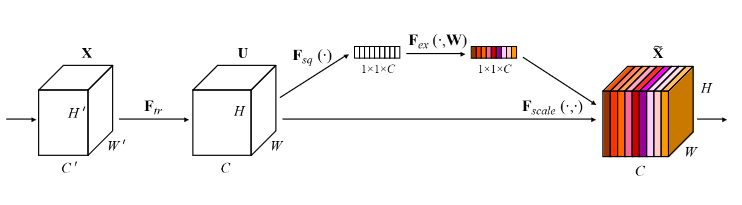
\includegraphics[scale=0.45]{src/BackgroundReading/assets/squeze_and_excitation.png}
    \caption{Squeeze-and-Excitation block architecture}\label{fig:squeze_and_excitation}
\end{figure*}

This type of CNN is a transitional link between classical CNN architecture 
and transformer architecture in CV~\cite{transformers}.
Authors of the paper\cite{seNet} propose a Squeeze-and-Excitation block that performs as 
attention mechanism that can be embedded in CNN architecture.

The main idea is to flatten each channel of the input feature map in a such way, 
that each channel would be represented by only one value. It can be done by
applying global average pooling to each channel:
\[F_{sq}(u_c) = z_c = \frac{1}{H\cdot W} \cdot \sum\limits_{i=1}^H\sum\limits_{j=1}^W u_c(i,j)\]
where $u_c$ \- input channel, $W$ and $H$ are spatial dimensions, $z_c$ \- result statistic

After that, it's needed to implement nonlinear interaction between channels, to do that
it's a good idea to use 2 fully connected layers, one with ReLU activation and the other
with simple sigmoid:
\[F_{ex}(z,W)=s = \sigma (W_2\cdot (\delta(W_1\cdot z)))\] 
where $z$ embeddings from previous step, $W_1 \in \mathbb{R}^{\frac{C}{r}\times C}$, 
$W_2 \in \mathbb{R}^{C \times \frac{C}{r}}$, $\sigma$ \- ReLU activation.

$r$ is a scale factor: fully connected layers are computationally heavy, so decreasing the
hidden layer is needed for optimization purposes.

Finally, $s$ should be scaled up to save spatial dimensions of input, to achieve this the input of the block can be multiplied on $s$ channel-wise:
\[F_{scale}(u_c)=\widetilde{x}_c = s_c \cdot u_c\]

The full architecture is shown in Figure~\ref{fig:squeze_and_excitation}.

This approach can be implemented in any architectures described above, it's 
computationally lightweight and gives a good accuracy boost ($1.7\% $ for MobileNet 
and $1.4\%$ for EfficientNet).

\subsubsection{General ideas}
Also important to mention, that all the described above approaches can't be 
implemented directly due to a lack of computational resources, so only its ideas 
will be taken. Such layers like batch normalisation\cite{batch_norm} or dropout\cite{dropout} also will be used,
because they prevent overfitting and let models converge faster, which is important,
due to the low size of the dataset.

\section{Project planning}
\subsection{Introduction}
The project was divided into three main steps:
\begin{enumerate}
    \item Preparing the dataset.
    \item Choosing and implementing deep learning model.
    \item Deploying model on the Duckiebot.
\end{enumerate}
Each step was a small project with its research, implementation and evaluation. 
\subsection{Methodology}
\subsubsection{Intorduction}
I haven't intentionally used any specific methodology or Agile techniques except MoSCoW, 
because, in my opinion, it is nothing but a waste of time. However, it happened that I had some kind of scrum sprints.
Each step described above was made as a scrum sprint of two weeks of 14 hours of work per day.
\begin{table}[h]
    \centering 
    \begin{tabular}{|p{1.7cm}|p{6cm}|p{6cm}|}
        \hline
        Priority & Description & Result \\ \hline
        Must & Design, develop and deploy algorithm using reinforcement learning technique for marking up dataset & Dataset collected, algorithm published \\ \hline
        Must & Design and develop a light-insensitive and light-weight algorithm for detecting road marking & Algorithm developed and published \\ \hline
        Should & Deploy light insensitive and light-weight algorithm for detecting road marking on Duckeibot & Algorithm deployed, full built is published  \\ \hline
        Could & Crossroad crossing algorithm based on computer vision techniques & Algorithm hasn't been developed, 
        but it can be after finishing all the exams. In this case, the algorithm would be published as a scientific paper \\  \hline
        Won't be & Light-weight general-purposes line detection algorithm, which can be used for any type of road markup & Algorithm hasn't been developed and won't be
        developed by me during spring-summer 2024\\ \hline
    \end{tabular}
    \caption{MoSCoW table with the results}\label{tab:MoSCoW}
\end{table}
\subsubsection{Preparing dataset}
The preparation of the dataset was divided into five substeps fully described in the design and implementation chapters:
\begin{enumerate}
    \item Writing some utilities for getting pictures from the Duckiebot.
    \item Collecting dataset.
    \item Research on self-supervised learning techniques for marking up the dataset.
    \item Creating a self-supervised learning model and pipeline for marking up the dataset.
    \item Validation of the resulted markup by a human.
    \item Publishing the dataset.
\end{enumerate} 
\subsubsection{Choosing and implementing deep learning model}
This step was just a classical example of the creation of a DL model. So it was divided into 2 substeps:
\begin{enumerate}
    \item Reading articles.
    \item Model implementation.
\end{enumerate}
\subsubsection{Deploying model on the Duckiebot}
The last step of the project was also divided into 3 substeps:
\begin{enumerate}
    \item Running DL model on the Duckiebot.
    \item Adjust the outputs of the model in a such way that they fit the inputs of the lane-following algorithm of the base docker image of the Duckiebot.
    \item Evaluate the result of the deployment and the whole project.
\end{enumerate}
\subsection{Requirements}
\subsubsection{Preparing dataset}
For this part of the project, there were 2 requirements:
\begin{enumerate}
    \item Collect about 9000 photos for the dataset. In the flat, where the polygon was mounted, there are 2 sets of lamps, so 3000 photos per set were collected, 
    as well as 2000 photos for the combination of the sets and 1000 photos with daylight only.
    \item Create a self-supervised learning algorithm for marking up the dataset with an accuracy of at least 70\%. 
\end{enumerate}

The first requirement is needed to make resulted algorithm light-insensitive. With a combination of data augmentation 
(to be more precise color and brightness shifting) the dataset collected in a such way can make the resulting DL model pretty accurate, because
it will not rely only on the colors and brightness of pixels in its predictions (this will be shown in the implementation chapter).

The second requirement was partly my interest and partly project requirements. For me, it was interesting to learn how to segment a picture on colors in different 
light conditions. For the project, it was important to have a pretty large dataset to train the DL model on.

\textbf{Human validation}

As a result, of implementing this part of the project one more requirement was found. It is human validation of the dataset.

Human validation is a critical step in creating a road marking dataset (even for Duckietown, which cannot harm a person), the marking of which was created automatically. 
A human can ensure the accuracy and reliability of the data obtained, which is extremely important in the autopilot contest.
Unlike machine learning algorithms without a teacher, people are able to recognize inaccuracies in machine markup: incorrect classification, noise and 
other artifacts. Human verification of the markup, although it reduces the size of the dataset, improves the average quality of the markup, 
reducing the risk of incorrect training of the neural network, and thereby improving autopilot in real conditions.

Human verification reduces the overall noise of the dataset. This provides an opportunity to get better training data for deep learning algorithms.
With careful verification, a person is able to eliminate false labeling and correct falsely labeled pixel maps, thereby ensuring semantic consistency
throughout the dataset. This noise reduction has a beneficial effect on the training of neural networks, especially on relatively small datasets for 
computer vision.

Even though human verification entails additional financial expenses and consumes a lot of time, its necessity is priceless, especially for
datasets on which machine learning algorithms are trained, the results of which can harm a person. Human verification allows you to overcome the limitations
associated with automatic markup, such as false segmentation or noise, which can lead to incorrect training, and then the operation of the neural network.
In the case of using neural networks for autopilot operation, incorrect operation of the algorithm can lead to human casualties.

Last but not least. The project used human verification of automatic markup, rather than fully human markup. This approach allows, on the one hand, 
to ensure the accuracy of the dataset, and on the other hand, it does not require resources such as completely human markup. Although this approach slightly
reduces the size of the dataset, it is a reasonable compromise combining both human precision and the scalability that automatic markup provides.
This approach allows, using limited resources, to create large and relatively accurate datasets, which is very important in such computer
vision algorithms.

\subsubsection{Choosing and implementing deep learning model}
For this step, requirements were hardly evaluated, because some characteristics of the model (e.g.\ time per froward pass) are different in a training environment 
(Gooogle Colab) and working environment (the Duckiebot). So the requirements of this part of the project can be implemented and evaluated in different steps.
\begin{enumerate}
    \item Model should be pretty small. I assumed the volume of all the parameters of the model can't be more than 2GB (even thou the Duckiebot has 4GB of RAM I've 
    decided to leave some space for other parts of the OS).
    \item Model should be fast. The forward pass of the model shouldn't take more than 20 milliseconds. This requirement is important to make enough FPS rates. 
    I assumed that having 20 FPS is more than enough for the Duckiebot. So if the model takes 20 milliseconds and data transferring takes 30 milliseconds this will 
    be 50 milliseconds per image which is 20 FPS.\@ In the Implementation chapter it will be described in more detail.
\end{enumerate}

\subsubsection{Deploying model on the Duckiebot}
In this part of the project, there were no requirements in the beginning, but when during the implementation, it was figured out that this task wasn't as easy as expected.
\begin{enumerate}
    \item Deploy the DL model to the Duckiebot and adjust the outputs of the model in a such way that they fit the inputs of the lane-following algorithm of the base 
    docker image of the Duckiebot. This was the only requirement at the beginning of the project.
    \item Migrate to TensorRT SDK.\@ This requirement appeared as soon as I ran the model on the Duckiebot 
    because without TensorRT SDK the forward pass of the model and the data transferring were much slower than I expected 
    (in more detail it is described in the Implementation chapter).
\end{enumerate}

\subsection{Potential Solutions}
\subsubsection{Introduction}
There can be a lot of variants of implementation of this project. I will divide this section into two subsections:
\begin{enumerate}
    \item Languages and libraries to discuss choices of the languages and libraries used in the project.
    \item Algorithms to discuss choices of the algorithms used in the project.
\end{enumerate}
\subsubsection{Languages and libraries}
\begin{enumerate}
    \item Language for the server to collect photos from the Duckiebot. Servers can be written in almost any language: Python, Java, NodeJS, etc. But I've decided 
    to use GoLang as I'm familiar with writing servers in this language. Because the server wasn't the main part of the project, but just a utility I didn't need it to 
    be extensible or super efficient. The only important thing about the server was quick development and GoLang can provide instruments for this in addition my knowledge
    of this language made it the only option for this project.
    \item Main language for the project. It's already standard for the industry to use Python as a language for the ML/DL projects~\cite{pythonForAI}, so for me, it 
    wasn't a question of which language to use. However important to mention that sometimes ML/DL projects can be written in RLang or MATLAB, but I'm not familiar
    with either of them, also MATLAB as far as I know isn't free to use, moreover, Duckietown uses Python as the main language. Also, it was possible to
    consider using C++ and writing the DL model in this language, but this would increase development time because I've never worked with Torch on C++ and have 
    no experience in developing ROS nodes for the Duckiebot in this language.
    \item Libraries for the project. Talking about libraries it's important to mention that there are almost no analogs for the Scikit-learn library which was used 
    for the EM algorithm. But for the DL model, there are two big analogs of the PyTorch library used in this project. These analogs are TensorFlow and JAX, which are 
    also libraries for creating neural networks. 
    However, I learned deep learning using PyTorch so I know this library much better than TensorFlow and JAX, moreover, the Duckietown project has no base docker images
    with JAX or TensorFlow so these libraries weren't even considered.
    
\end{enumerate}

\subsubsection{Algorithms}
\begin{table}[h]
    \centering 
    \begin{tabular}{|c|c|}
        \hline
        Model & Parameters \\ \hline
        My model & 10,5K \\ \hline
        DeepLabV3 & 11M  \\ \hline
        FCN & 35,3M \\  \hline
        LRASPP & 3,2M \\ \hline
    \end{tabular}
    \caption{Fully implemented NN in comparison with my architecture}\label{tab:nn_arcitecture}
\end{table}
\begin{enumerate}
    \item Using EM algorithm for marking up the Dataset. EM algorithm wasn't the only option for the marking up algorithm as it was described in 
    the Background reading chapter. Also in addition to that chapter, I considered using the DBScan algorithm in combination with the `energy approach'. 
    But the EM algorithm showed its consistency and it was decided to use it.
    \item DL architecture also has a lot of options as was described in the Background reading chapter. But the resulting algorithm was pretty consistent, light-weighted 
    in computational terms and had a relatively small amount of trainable parameters, so it was decided to stay on the created architecture. I thought about    using other 
    backbones like ShuffleNet~\cite{shufflenet}, EfficientNet~\cite{efficientnet} or Visual Transformers~\cite{transformers} or even fully implemented segmentation neural
    networks like DeepLabV3~\cite{deeplabv3}, FCN~\cite{FCN} or LRASPP~\cite{mobilenetv3}, but all these variants are either too big or too computationally heavy and do not 
    give much better results.
\end{enumerate}
\subsection{Tools and Techniques}
During this project, a lot of different tools were used:
\begin{enumerate}
    \item IDEs of JetBrains were used for developing:
    \begin{enumerate}
        \item PyCharm for Python developing.
        \item GoLand for GoLang development.
    \end{enumerate}
    \item Jupiter notebooks were used for developing ML algorithms (both the EM algorithm and the DL model). For the model training, Google Colaboratory was used, 
    because I don't have a computer with GPU to train my model on.
    \item Also usual in development things were used in my project:
    \begin{enumerate}
        \item git for VCS and GitHub for publishing results.
        \item Docker for deployment on the Duckiebot.
    \end{enumerate}
    \item Visual Studio Code was used for writing this report because it is written in \LaTeX. 
\end{enumerate}

\subsection{Legal, Social, and Ethical Issues}
\subsubsection{Intorduction}
As it was written in the technical plan (appendix 1) it is a research project with no legal, social or ethical issues. However, after the full implementation of
the project, some things need clarification.
\subsubsection{The dataset}
The Dataset was collected and published under MIT license~\cite{mit}. The choice of license is so because I want the dataset to be used by other users, but
because of autonomous marking up (even if the markup has been verified by a human), there can be some mismarked pictures, which can cause problems In training some 
algorithms. 
\subsubsection{The algorithm}
The algorithm is also published under MIT license~\cite{mit}. The reason is simple. I want the algorithm to be open-sourced and available for free commercial, 
educational or any other usage. The algorithm was developed for Duckiebot, but it can (but is not recommended to) be
used as a baseline for real autonomous driving cars. However, this usage of the algorithm wasn't initially planned that's why I don't want to be responsible for any consequences of
misusing my algorithm.
\subsubsection{The Duckiebot}
The Duckiebot can drive autonomously. So it can cause some legal issues if it bumps into something or someone. Even though the bot is small it can break something. 
That is the reason why it should be run only under human control to prevent such accidents. 

Also, the bot was provided for me by the University, so I'm responsible for its condition and possible damage, that's why running the bot without my control and permission 
was and remains strongly prohibited. 
\subsection{Summary}
This section was written after the project was finished so it shows not only planning but also the resulting technologies and ideas that were used.
As you can notice different approaches were considered and rejected, to fully satisfy the desired requirements. As it was said Agile wasn't intentionally used, 
but anyway the project was finished on time and it met all the requirements. A lot of different tools and programming languages were used in this project.
As it was said it is a research project that doesn't involve any people (besides me, the developer) and doesn't use unlicensed software, so it can't have any legal, 
ethical or social issues.
\section{Design}
\subsection{Introduction}
This chapter covers project architecture and process flow as well as the math foundations of algorithms used in this project.
The second topic is partly covered in the Background reading chapter, but here there is all the information necessary for understanding.
\subsection{Project architecture and process flow}
\begin{figure}[ht]
    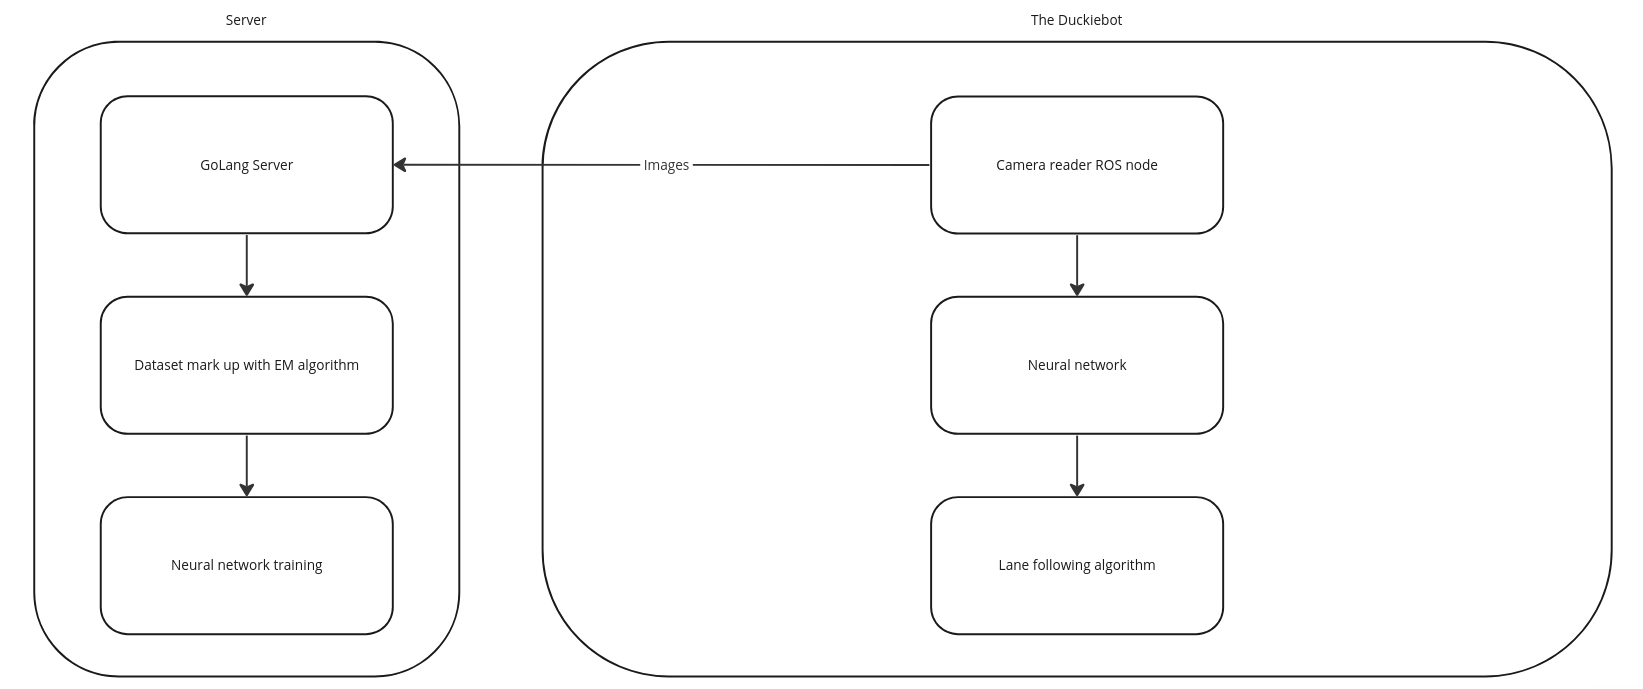
\includegraphics[scale=0.25]{src/Design/assets/ProjectArchitecture.png}
    \caption{Project architecture}\label{project_architecture}
\end{figure}
\subsubsection{Introduction}
As was written in the previous chapter the project was divided into three mini-projects:
\begin{enumerate}
    \item Creating the dataset.
    \item Creating road markup segmentation algorithm.
    \item Deployment of the algorithm on the Duckiebot.
\end{enumerate}
Each mini-project has its own architecture and process flow, however, they were developed in similar environments.
The overall environment is shown in Figure~\ref{project_architecture}. Pictures were collected from the Duckiebot's camera, then they were sent to the GoLang server. 
After that, they were processed in Google Colab and then passed to the neural network training pipeline. During the deployment part images from the same camera on the Duckiebot
were passed to the neural network which had been already deployed on the Duckiebot. And outputs of the neural network were passed to the lane-following algorithm.
\subsubsection{Creating the dataset}
Collecting the dataset involved three steps:
\begin{enumerate}
    \item Developing the infrastructure. The infrastructure includes the ROS node to send data from Duckiebot and the GoLang server to receive and save data. 
    The image was received from the camera and after that, it was sent to the server. Because sending takes some time and this process couldn't be run asynchronously,
    not all images were sent, but every 20.
    \item Collecting the dataset. The collecting of the Dataset was performed manually. The Duckiebot was driven around the road for a few hours. 
    During this process, the lights were changed to collect different data.
    \item Marking up the dataset. The marking up of the Dataset was performed in the Jupiter notebook. Images were marked up in batches of size no more than 500 samples.
    Moreover, pictures of the different light conditions were marked up in different iterations of the pipeline, to prevent noise. After the marking up the dataset was 
    evaluated by humans to remove samples with bad segmentation and after that uploaded to GitHub.
\end{enumerate}
\subsubsection{Creating road markup segmentation algorithm}
\begin{figure}[ht]
    \begin{center}
        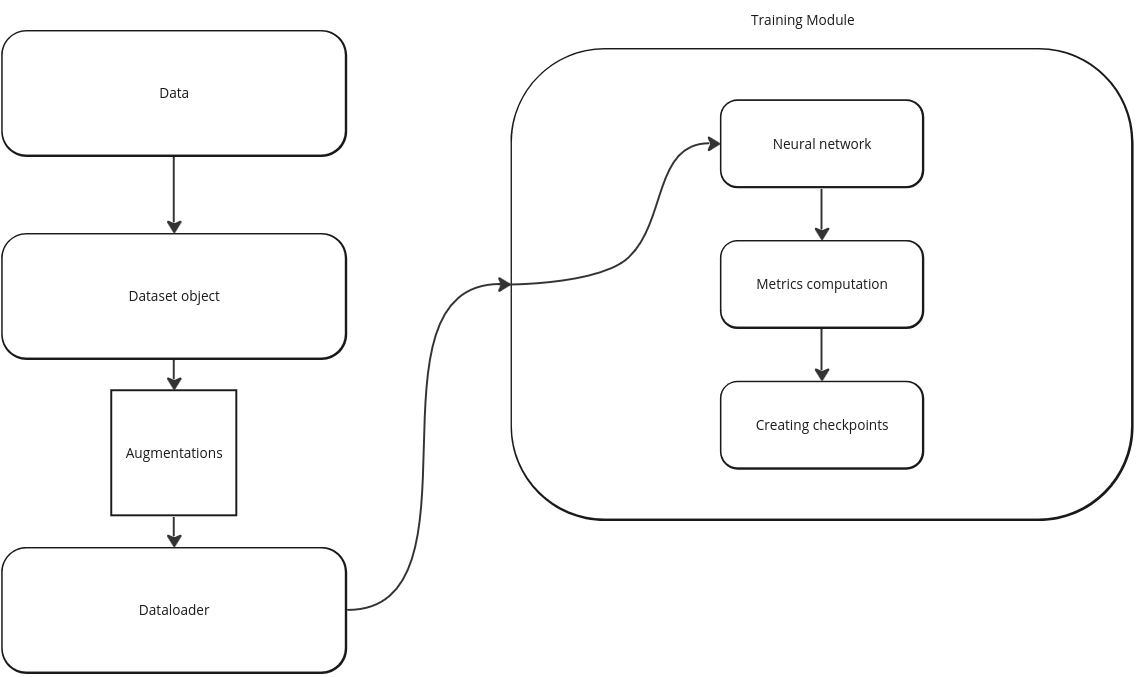
\includegraphics[scale=0.25]{src/Design/assets/TrainingPipeline.png}
    \end{center}
    \caption{Training pipeline}\label{training_pipeline}
\end{figure}
The algorithm was developed in the Jupiter notebook in Google Colab. The pipeline is shown in figure~\ref{training_pipeline}.

The dataset was downloaded from GitHub (it more quicker than uploading it to Colab from a laptop). After that, the data of the dataset was loaded into the dataset class.
The idea of this class is to keep information about the dataset, but not the data itself, because the dataset is pretty huge and keeping all data loaded in the RAM is pretty expensive.
So the Dataset class provides lazy access to the dataset data. If some sample is required it will be loaded, otherwise, only the path to the image will be saved. Also,
the Dataset class is responsible for the augmentation of the data. When a sample is required if this sample is part of the training part of the dataset, then the object 
of the Dataset class will return it with some augmentation, otherwise (if the sample is part of the validation or test part) it will be returned without augmentations.
The Dataset class is used in the Dataloader class. This class is responsible for creating batches of the data and shuffling the test part of the dataset. In this project, it is 
the only functional of the Dataloader class that was used. Whenever the neural network requires a new batch of data, it asks the Dataloader class for it, which uses the Dataset class to load
a few images and provide them to the neural network.

Batches received from the object of the Dataloader class are used in the training and validation of neural network. The TrainingModule class is responsible for this.
This class is developed to make training of the neural network easy. This class has a huge amount of functionality, however, in the project only a few things were used.
The object of the TrainingModule class is responsible for:
\begin{enumerate}
    \item Training the neural network for a few epochs, so the neural network will use in its training each sample of the training part of the dataset a few times.
    \item Calculating metrics during training and validation. It's extremely important because early stopping is used in the training pipeline.
    \item Creating checkpoints of the model. If the target metric of the model doesn't improve after a few epochs the training is finished and a few best iterations are saved.
\end{enumerate}
The overall process flow can be described like this:
\begin{enumerate}
    \item All images saved in Google Colab. All paths are saved in RAM.\@
    \item When an image is required for training or validation it is loaded into RAM.\@ If the image is part of the training part of the dataset augmentations are applied to it.
    \item Required images are combined into a batch.
    \item The batch is fed to the neural network.
    \item The metrics of the batch are computed.
    \item Weights of the neural network are adjusted based on metrics.
    \item When all images of the training part of the set are used (it's called epoch), the images of the validation part are fed to the neural network.
    \item The metrics of the validation part are computed.
    \item If the metrics of validation part don't improve after a few epochs training stops.
    \item The neural network is validated on the test part of the dataset. 
\end{enumerate}

\subsubsection{Deployment}
\begin{figure}[ht]
    \begin{center}
        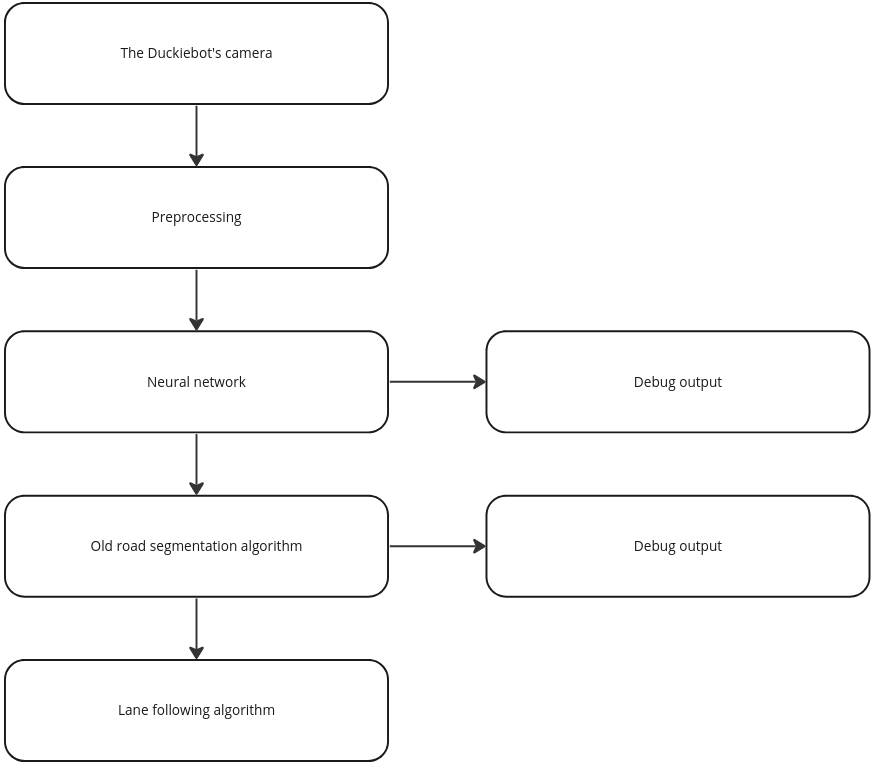
\includegraphics[scale=0.25]{src/Design/assets/Deployment.png}
    \end{center}
    \caption{Deployment}\label{deployment}
\end{figure}
The resulting architecture that is used on the Duckeibot is shown in figure~\ref{deployment}. The image received from the camera of the Duckiebot is preprocessed.
The upper part of the image is removed, because usually it doesn't contain road. After that image is converted to a torch-GPU-tensor. Then this tensor is fed to the neural network.
The output of the neural network is fed into the old lane segmentation algorithm, to convert the output of the neural network to the input of the lane-following algorithm.
The result is fed to the lane-following algorithm, which controls the Duckiebot's movements based on the road markup.

It was decided to use the old lane segmentation algorithm to increase the speed of the development and reduce the risk of creating bugs. However, the old algorithm isn't
fully used. Only the part that is responsible for converting the pixel map to a special input format of the lane-following algorithm is used. The part of creating pixel 
map is removed, because this functionality is taken by the neural network, which was the initial goal of the project.

Also important to mention that the output of the neural network (pixel map) and old lane segmentation (segments of road markup) are sent to a special debug ROS node, which can 
visualize in real-time the images produced by these algorithms. To create these pictures some time is required, so if the debug node isn't used 
(the window with debug information isn't opened) these images won't be sent, which saves some time.
\subsection{EM algorithm}
\subsubsection{Simple case}
Assume there are some amount of points in d-dimensional space, they are samples. The task is to segment them.
\begin{figure}[ht]
    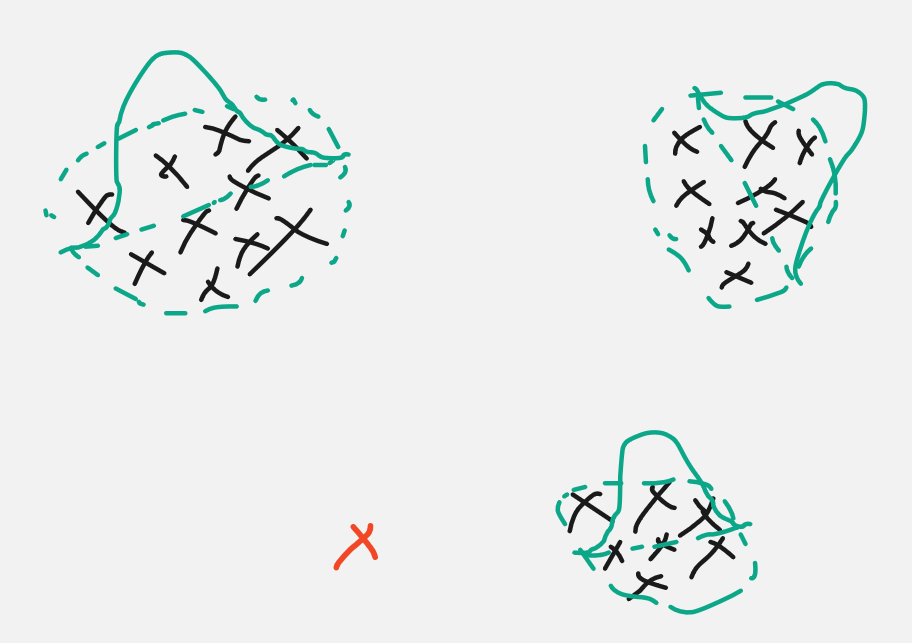
\includegraphics[scale=0.5]{src/Design/assets/em_picture.png}
    \caption{Data visualisation}
\end{figure}
Assume that the picture above is generated by a mixture of three Gaussians.
\[p(\overline{x}) = \pi_1\cdot p_1(\overline{x}) + \pi_2\cdot p_2(\overline{x}) + \pi_3\cdot p_3(\overline{x}) \]
where
\[\sum\limits_{k=1}^{K} \pi_k = 1 \text{ where } K=3\]
In other words, with probability $\pi_i$ Gaussian is chosen and after that, the sample is generated based on this Gaussian 
$\overline{x} \sim p_k(\overline{x})$.
But how to classify a new point (the red one)?
The likelihood function is required:
\[p(D|\overline{\theta}) = \prod\limits_{n=1}^N p(\overline{x}_n | \overline{\theta}) \text{ here D means whole dataset, in other words } D = \{\overline{x}_n \} _{n=1}^N\]
Where
\[p(\overline{x} | \overline{\theta}) = \sum\pi_k\cdotp_k(\overline{x}) = \sum\limits_{k}\pi_k\cdot\mathcal{N}(\overline{x}|\overline{\mu}_k, \Sigma_k)\]
\[\text{Where } \overline{\mu}_i \text{ and } \Sigma_i \text{ are parameters of PDF of normal distribution and } \overline{\theta} = (\pi_1, \dots \pi_K,
\overline{\mu}_1, \Sigma_1, \dots, \overline{\mu}_K, \Sigma_K)\] 
So after that:
\[p(D|\overline{\theta}) = \prod\limits_{n=1}^N p(\overline{x}_n | \overline{\theta}) =
 \prod\limits_{n=1}^N (\pi_1\cdot p_1(\overline{x}_n | \overline{\theta}_1) + \pi_2\cdot p_2(\overline{x}_n | \overline{\theta}_2) + 
 \dots + \pi_K\cdot p_K(\overline{x}_n | \overline{\theta}_K) ) \overset{}{\underset{\overline{\theta}}{\rightarrow}} \text{max}\]
 Where $\overline{\theta}_i = (\overline{\mu}_i, \Sigma_i)$

The problem is that it is a multiplication of a big amount of sums which is difficult to optimize.
The idea is to look at the distribution, likelihood and generation process and think about what other information about this process is required to make 
the likelihood function easy to optimize.

It turns out that adding to the $\overline{x}$ label of its class makes everything much easier. In math terms:
\[ Z = \{\overline{z}_n \} _{n=1}^N \text{, where each } \overline{z}_n \text{ is one-hot encoded: } \overline{z}_n = (0,\dots,1,\dots0)\] 
and only 1 of this vector is on the kth position, which means that $x_n \in C_k$, where $C_k$ means cluster number k.
So if $Z$ is known, then 
\[p(D, Z | \overline{\theta}) = \prod\limits_{n=1}^{N}p(\overline{x}_n, \overline{z}_n | \overline{\theta})
= \prod\limits_{n=1}^{N}p(\overline{z}_n | \overline{\pi})\cdot p(\overline{x}_n| \overline{z}_n, \overline{\theta})
= \prod\limits_{n=1}^{N}\prod\limits_{k=1}^{K}{(\pi_k\cdot\mathcal{N}(\overline{x}_n|\overline{\mu}_k,\Sigma_k))}^{{z_n}_k}\]
Now it's good practice to take the logarithm of likelihood function because it transforms the product into a sum which is a more convenient operation to work with
\[\log(p(D, Z | \overline{\theta})) = \sum\limits_{n=1}^{N}\sum\limits_{k=1}^{K}{z_n}_k \cdot (\log(\pi_k) +  \log(\mathcal{N}(\overline{x}_n|\overline{\mu}_k,\Sigma_k)))
= \sum\limits_{k=1}^K \log(\pi_k) \cdot \sum\limits_{n=1}^N {z_n}_k + 
\sum\limits_{k=1}^K \big( \sum\limits_{n=1}^N {z_n}_k \cdot \log(\mathcal{N}(\overline{x}_n|\overline{\mu}_k,\Sigma_k)) \big)\]
Now important to notice that the first and the second summands depend on different parameters.
The first summand depends on $\pi_k$, while the second depends on parameters of PDF of normal distribution $\overline{\mu}_k, \Sigma_k$. So it's possible to optimize these summands separately.

And now the main idea. There is a complicated likelihood function with latent variables that are not known, but if they were everything would be easy. 
So the idea is to split the process into two steps:
\begin{enumerate}
    \item E-step (fix $\overline{\theta}$, find $\mathbb{E}[Z]$):
    \[\mathbb{E}[z_{n, k}] = p(C_k|\overline{x}_n,\overline{\theta}) 
    = \displaystyle \frac{p(C_k|\overline{\theta})\cdot p(\overline{x}_n|C_k,\overline{\theta})}{\sum\limits_{l=1}^K p(C_l|\overline{\theta})\cdot p(\overline{x}_n|C_l,\overline{\theta})}
    = \displaystyle \frac{\pi_k\cdot \mathcal{N}(\bar x_n | \bar \mu_k, \Sigma_k)}{\sum\limits_{l=1}^K \pi_l \cdot \mathcal{N}(\bar x_n | \bar \mu_l, \Sigma_l)}\]
    \item M-step (fix $\mathbb{E}[Z]$, maximize $\mathbb{E}[\log(p(D,Z|\overline{\theta}))]$). In most cases, instead of $Z$, we can use soft estimates $\mathbb{Z}$:
    \[\mathbb{E}[\log p(D,Z|\bar\theta)] 
    = \mathbb{E}\Big[\sum\limits_n\sum\limits_k {z_n}_k \cdot \big(\log(p(\overline{x}_n|\overline{\mu}_k, \Sigma_k)) + \log(\pi_k)\big)\Big]\] 
    \[ = \sum\limits_n\sum\limits_k\mathbb{E}[{z_n}_k]\cdot(\log(\pi_k) + \log\big(p(\overline{x}_n|\overline{\mu}_k, \Sigma_k))) \newline
    = \sum\limits_k\Big(\sum\limits_n\mathbb{E}[z_{n,k}]\Big) \log \pi_k + \sum\limits_k\sum\limits_n\mathbb{E}[z_{n,k}]\cdot \log p(\bar x_n|\bar\mu_k,\Sigma_k)\]
\end{enumerate}

\subsubsection{General case}
There are:
\begin{enumerate}
    \item X \- the dataset
    \item Z \- latent variables we don't know them
    \item $\theta$ \- parameters we also don't know them
\end{enumerate}
The goal is to maximize $p(X|\theta)$, which is a complicated task, but optimizing $p(X, Z|\theta)$ is easier. So let
\[Q(\theta, \theta^{(n)}) := \mathbb{E}_{p(Z|X,\theta^{(n)})} \big[\log p(X,Z|\theta)\big]
= \int \log p(X,Z|\theta) \cdot p(Z|X,\theta^{(n)}) dz \]
And on each step:
\[\theta^{(n+1)} = \underset{\theta}{argmax}Q(\theta, \theta^{(n)})\]

These steps are executed until $\theta$ stops changing or the likelihood function stops changing (theoretically it should happen simultaneously). 
Also, the likelihood function should increase after each step. So in the end:
\[\log(p(X|\theta)) > \log(p(X|\theta^{(n)}))\]
\[\log(p(X|\theta)) - \log(p(X|\theta^{(n)})) 
= \log \Big( \int p(X,Z|\theta) dz \Big) - \log(p(X|\theta^{(n)})) \]
\[= \log \Big(\int p(Z|X,\theta^{(n)} \cdot \displaystyle \frac{p(X,Z|\theta)}{p(Z|X,\theta^{(n)})}) dz \Big) - \log(p(X|\theta^{(n)}))\]
\[= \log\Big( \mathbb{E}_{p(Z|X,\theta^{(n)})}\big[\displaystyle\frac{p(X,Z|\theta)}{p(Z|X,\theta^{(n)})} \big] \Big) - \log(p(X|\theta^{(n)})) \]
\[ \underset{\text{by the Jensen's inequality}}{\geq} \mathbb{E}_{p(Z|X,\theta^{(n)})}\Big[\log\big(\displaystyle\frac{p(X,Z|\theta)}{p(Z|X,\theta^{(n)})} \big) \Big]  - \log(p(X|\theta^{(n)})) \]
\[ = \mathbb{E}_{p(Z|X,\theta^{(n)})}\Big[\log\big(\displaystyle\frac{p(X,Z|\theta)}{p(Z|X,\theta^{(n)}) \cdot p(X|\theta^{(n)})} \big) \Big]\]
Now important to notice, that $p(Z|X,\theta^{(n)}) \cdot p(X|\theta^{(n)}) = p(X,Z|\theta^{(n)})$

\noindent And therefore:
\[ \log(p(X|\theta)) \geq \log(p(X|\theta^{(n)})) + \mathbb{E}_{p(Z|X,\theta^{(n)})}\Big[\log\big(\displaystyle\frac{p(X,Z|\theta)}{p(Z|X,\theta^{(n)}) \cdot p(X|\theta^{(n)})} \big) \Big] =: \mathcal{L}(\theta, \theta^{(n)})\]

\begin{figure}[h]
    \begin{center}
        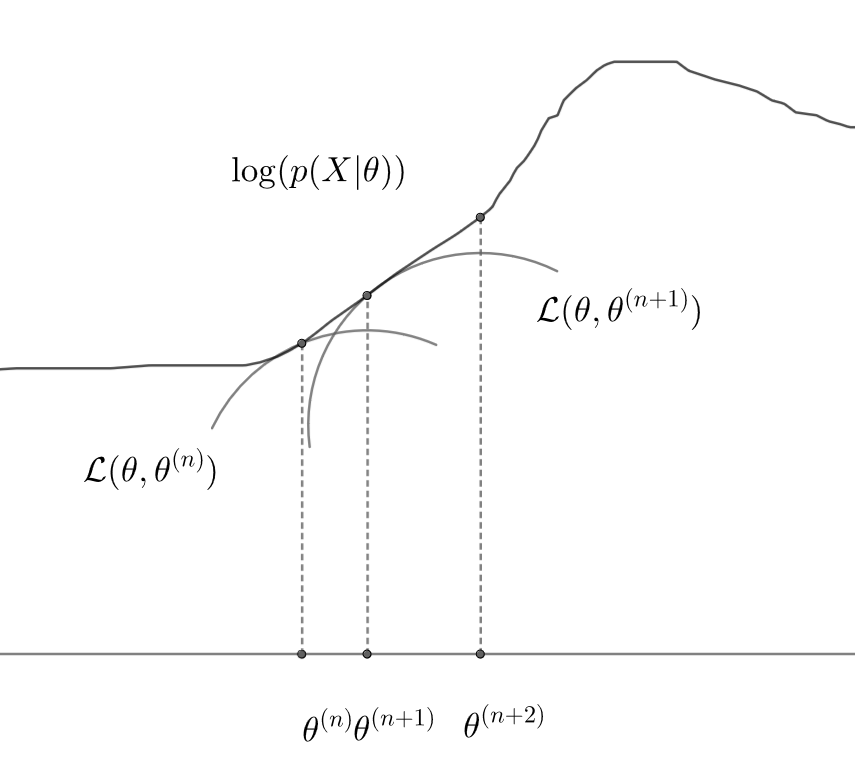
\includegraphics[scale=0.45]{src/Design/assets/em_visualisation.png}
    \end{center}
    \caption{Algorithm visualisation}
\end{figure}

As shown in the picture in each point ($\theta^{(n)}$, $\theta^{(n+1)}$, $\theta^{(n+2)}$, etc) the lower score of $\log(p(X|\theta))$ is known. This score is $\mathcal{L}(\theta, \theta^{(n)})$

Also, it's important to mention that $\log(p(X|\theta^{(n)})) = \mathcal{L}(\theta^{(n)}, \theta^{(n)})$

So the idea is to optimize $\mathcal{L}(\theta, \theta^{(n)})$. The function converges to a local maximum which is also good.

But in the beginning, it was said that $Q(\theta, \theta^{(n)})$ needs to be optimized, it turns out that in terms of optimization $Q$ and $\mathcal{L}$ 
are the same functions.

\[ \mathcal{L}(\theta, \theta^{(n)}) = \underset{const(\theta)}{\log(p(X|\theta^{(n)}))} + \underset{\text{it is } Q(\theta, \theta^{(n)})}{\mathbb{E}_{p(Z|X,\theta^{(n)})}\Big[\log\big(p(X,Z|\theta) \big) \Big]}
- \underset{const(\theta)}{\mathbb{E}_{p(Z|X,\theta^{(n)})}\Big[\log\big(p(X,Z|\theta^{(n)})\big)\Big]}
    \]

\subsection{Deep learning model}
\subsubsection{Architecture}
\begin{figure}[h]
    \begin{center}
    \subfloat[Full model architecture]{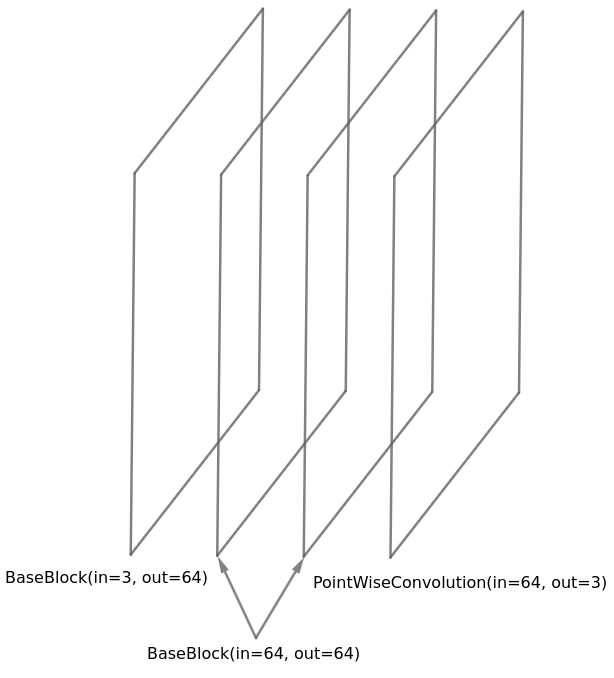
\includegraphics[scale=0.35]{src/Design/assets/nn_architecture.png}}
    \subfloat[Basic block architecture]{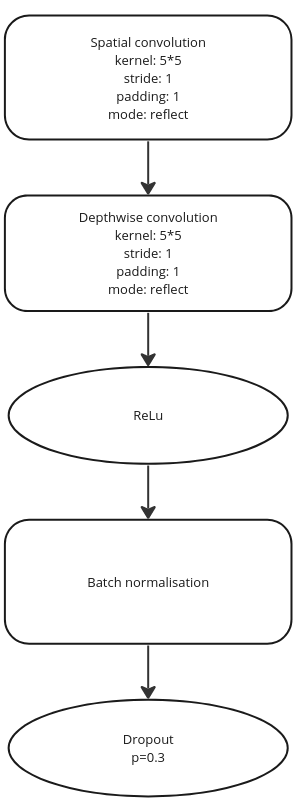
\includegraphics[scale=0.45]{src/Design/assets/basic_block_architecture.png}}
    \end{center}
    \caption{The DL model architecture}\label{nn_architecture}
\end{figure}
The architecture of the model is shown in Figure~\ref{nn_architecture}. The idea of MobileNet~\cite{mobileNet} for splitting the convolutional layer into two parts 
was used to increase the speed of the neural network.
As the loss function, the cross-entropy function was used.
\[ \mathcal{L}(x,y) = \{l_1,\dots,l_n\}; l_n=-w_{y_n}\log\frac{e^{x_{n,y_n}}}{\sum\limits_{c=1}^C e^{x_{n,c}}}\]
\[\text{ where } x\in \mathbb{R}^{n\times C} \text{ are outputs of the model}
\text{ and } y \in \mathbb{N}^n \text{ are ground truth class labels for each sample} \]

For the road markup segmentation task, this architecture was enough. Scores of the model are shown in the Implementation chapter. 
Each layer is described in more detail below.
\subsubsection{General neural networks ideas}
\begin{figure}[h]
    \begin{center}
    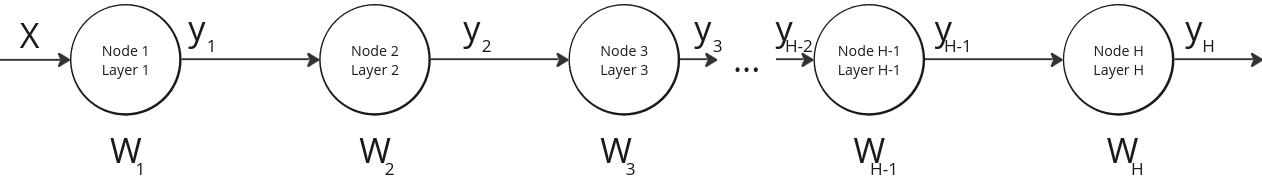
\includegraphics[scale=0.35]{src/Design/assets/computational_graph.png}
    \end{center}
    \caption{Computational graph}\label{com_graph}
\end{figure}
To talk about convolutional neural networks it's important to discuss the idea of neural networks in general.

Each neural network can be represented as a computational graph. The first node of the graph is the input and the last is the output of the network.
The output of the neural network (in formulas $\hat{y}$ is used) passes to the loss function. Almost always the task of training is to minimize the loss function.
To do this backpropagation is used.
Let $X \in \mathbb{R}^{n\times d}$ is input of the neural network, $\hat{y}\in \mathbb{R}^{n\times k}$ is output, $\{\hat{y}_i \in \mathbb{R}^{n \times k_i}\} _{i=1}^{H}$ 
is the output of the ith layer (or node in terms of the graph) of the neural network and $y \in \mathbb{R}^{n\times m}$ is a vector of ground truth answers 
(real numbers, class labels, etc). Also each layer has weights $\{ w_i \in \mathbb{R}^{k_i} \} _{i=1}^{H}$ (bias is included in weights for convenience) 
Here $n$ is used as the size of a dataset used for training and $H$ is the number of layers of a neural network (or nodes in terms of a graph)

In the described terms backpropagation can be described like this:
\begin{itemize}
    \item $\displaystyle\frac{\partial L}{\partial \hat{y}} =: \frac{\partial L}{\partial y_H}$ is the partial derivative of the loss function by the output of the neural network
    \item $\displaystyle \forall i \in \{1\dots H-1\}\text{ } \frac{\partial L}{\partial y_i} = \frac{\partial L}{\partial y_{i + 1}} \cdot \frac{\partial y_{i + 1}}{\partial y_i}$
\end{itemize}
The training is an iterative process, so $w_i^{(j)}$ mean weights of layer $i$ on the jth iteration of the process. The process can be described like this:
\begin{itemize}
    \item $\displaystyle \forall i \in \{2\dots H\} \text{ }w_i^{(j+1)} = w_i^{(j)} - \eta \cdot \frac{\partial L}{\partial w_i} \Big|_{w_i^{(j)}, y_{i-1}}$
    \item $\displaystyle w_1^{(j+1)} = w_1^{(j)} - \eta \cdot \frac{\partial L}{\partial w_1} \Big|_{w_1^{(j)}, X}$
\end{itemize}

All gradients and things specific to each layer used in the provided architecture are listed below

\subsubsection{Convolutional layer}
The convolutional layer is called this way because this layer performs a math transformation called convolution:
\[(f * g)(x) := \int\limits_{\mathbb{R}^n}f(x-y)g(y)dy= \int\limits_{\mathbb{R}^n}f(y)g(x-y)dy\]
However, in convolutional neural networks (CNN) this operation is usually performed iteratively because it's more efficient.
To implement the convolutional layer iteratively the sliding window is used.

Let $X \in \mathbb{R}^{N\times D \times H \times W}$ be the batch of input images (or feature maps) if it is an image $D$ usually equals $3$ and means the number of colors channels, 
$W$ and $H$ are the widths and the heights of the image or feature map and $N$ is the batch size (amount of samples of training set simultaneously fed to a neural network in 
a single forward pass).
$K = \in \mathbb{R}^{L \times D \times H_k \times W_k}$, where $W_k = 2\cdot a+1$ and $H_k = 2\cdot b+1$ is the kernel (sliding window).

The convolution of $X$ and $K$ ($X*K$) is another tensor $Y\in \mathbb{R}^{N\times L\times W' \times H'}$, where~\cite{conv2dTorch} 
\[
    W' = \displaystyle \Big\lfloor\frac{W  + 2 \cdot p_1 - d_1 \cdot (W_k - 1) - 1}{s_1} + 1\Big\rfloor    
\]
\[
    H' = \displaystyle \Big\lfloor\frac{H  + 2 \cdot p_0 - d_0 \cdot (H_k - 1) - 1}{s_0} + 1\Big\rfloor       
\]

\begin{figure}[h]
    \begin{center}
    \subfloat[Padding = 1]{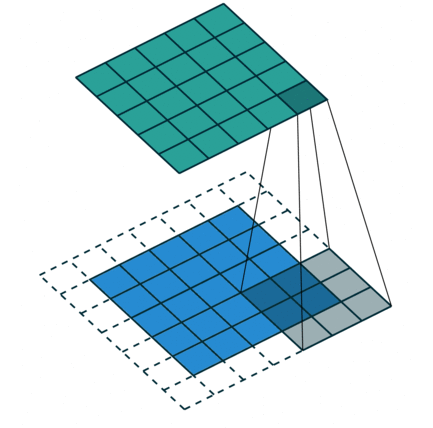
\includegraphics[scale=0.35]{src/Design/assets/padding.png}}
    \subfloat[Dilation = 2]{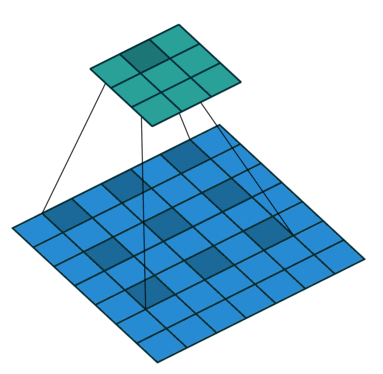
\includegraphics[scale=0.45]{src/Design/assets/dilation.png}}
    \\
    \subfloat[Stride = 2 (a)]{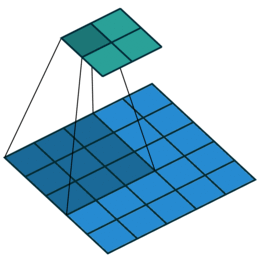
\includegraphics[scale=0.45]{src/Design/assets/stride1.png}}
    \subfloat[Stride = 2 (b)]{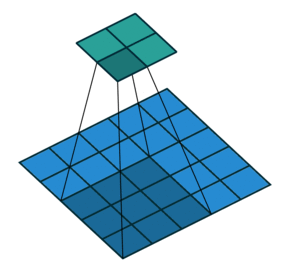
\includegraphics[scale=0.45]{src/Design/assets/stride2.png}}
    \end{center}
    \caption{Visualisation of convolution layer parameters}\label{conv2dparams}
\end{figure}

\begin{itemize}
    \item $p_i$ padding of spatial dimensions of the input tensor
    \item $d_i$ is dilation. Spacing between kernel elements
    \item $s_i$ is stride. A stride of the convolution
\end{itemize}

The visualisation of each parameter is shown on Figure~\ref{conv2dparams}~\cite{conv2dParamsArticle}

The elements of the result tensor are computed in the following way:
\[
    Y_{n, k, h, w} = \sum\limits_{d=0}^{D}\sum\limits_{j=-\lfloor W_k / 2\rfloor}^{\lfloor W_k / 2\rfloor}\sum\limits_{i=-\lfloor H_k / 2\rfloor}^{\lfloor H_k / 2\rfloor}
    X_{n, d, h \cdot s_0 + i \cdot d_0, w \cdot s_1 + j \cdot d_1} \cdot K_{k, d, i + \lfloor H_k / 2\rfloor, j + \lfloor W_k / 2\rfloor}
\]

The gradients of this layer can be computed like this (only the most common case, where $\displaystyle p_0 = \Big\lfloor \frac{H_k}{2} \Big\rfloor$, $\displaystyle p_1=\Big \lfloor \frac{W_k}{2} \Big\rfloor$ 
and $s_0 = s_1 = d_0 = d_1 = 1$ is considered because only this case was used in the project's architecture, important to notice that in this case $W'=W$ and $H'=H$):
\begin{itemize}
    \item To compute $\frac{\partial L}{\partial X}$ it's need to define $\widehat{K} \in \mathbb{R}^{D \times L \times W_k \times H_k}: \text{ } \widehat{K}_{d,l,w,h} = K_{l,d,h,w}$
    \[
        \displaystyle \frac{\partial L}{\partial X} = \frac{\partial L}{\partial Y} * \widehat{K}
    \]

    \item Some kind of convolution is also used to calculate $\frac{\partial L}{\partial K}$, but summation takes place by the size of the batch, not by channels 
    \[
        \frac{\partial L}{\partial K}_{l, d, h, w} = \sum\limits_{n=0}^N\sum\limits_{i=0}^H\sum\limits_{j=0}^W X_{n,d,i+h-\lfloor \frac{H_k}{2} \rfloor, j+w-\lfloor \frac{W_k}{2} \rfloor}
        \cdot \frac{\partial L}{\partial Y}_{n, l, i, j}
    \]
\end{itemize}

\textbf{Important notice} \\
$X_{i,-1,-1}$ is valid notation. It means that padded values are used. The mode of padding can be different in this project reflect mode is used.

\subsubsection{Batch normalisation layer}
This type of layer was first introduced in 2015 in this paper~\cite{batch_norm}.
This layer is used to keep all data in a neural network in one type of distribution. This technique prevents gradient explosions and 
helps a neural network to converge faster.
The idea of the batch normalization layer is pretty simple. During training update count mean and variance for the batch and apply it to training data and during inference just 
apply running estimates of those values to the data.

The forward pass of the layer during training can be described in the following way:
\begin{enumerate}
    \item Count batch statistics:
    \begin{itemize}
        \item $\mu = \displaystyle \frac{1}{m} \sum\limits_{i=1}^m x_i$
        \item $\sigma^2 = \displaystyle \frac{1}{m} \sum\limits_{i=1}^m (x_i - \mu) ^ 2$
    \end{itemize}
    \item Normalize the batch: $\hat{x_i} = \displaystyle \frac{x_i - \mu}{\sqrt{\sigma^2 + \varepsilon}}$
    \item Scale the batch: $y_i = \gamma \cdot \hat{x_i} + \beta$, where $\gamma$ and $\beta$ are trainable parameters
\end{enumerate}

During inference instead of $\mu$ and $\sigma^2$ $E[x]$ and $VAR[x]$ are used which were calculated during training.

Gradients of this layer are pretty simple:
\begin{enumerate}
    \item $\displaystyle \frac{\partial L}{\partial \hat{x}_i} = \frac{\partial L}{\partial y_i} \cdot \gamma$
    \item $\displaystyle \frac{\partial L}{\partial \sigma^2} = \sum\limits_{i=1}^m \frac{\partial L}{\partial \hat{x}_i} \cdot (x_i - \mu) \cdot \frac{-1}{2} \cdot
    {(\sigma^2+\varepsilon)}^{\frac{-3}{2}}$
    \item $\displaystyle \frac{\partial L}{\partial \mu} = \Big(\sum\limits_{i=1}^m \frac{\partial L}{\partial \hat{x}_i} \cdot \frac{-1}{\sqrt{\sigma^2 + \varepsilon}}\Big)
    + \frac{\partial L}{\partial \sigma^2 } \cdot \frac{\sum\limits_{i=1}^m -2(x_i-\mu)}{m}$
    \item $\displaystyle \frac{\partial L}{\partial x_i} = \frac{\partial L}{\partial \hat{x}_i} \cdot \frac{1}{\sqrt{\sigma^2 + \varepsilon}} +
    \frac{\partial L}{\partial \sigma^2} \cdot \frac{2(x_i-\mu)}{m} + \frac{\partial L}{\partial \mu} \cdot \frac{1}{m}$ 
    \item $\displaystyle \frac{\partial L}{\partial \gamma} = \sum\limits_{i=1}^m\frac{\partial L}{\partial y_i} \cdot \hat{x}_i$
    \item $\displaystyle \frac{\partial L}{\partial \beta} = \sum\limits_{i=1}^m\frac{\partial L}{\partial y_i}$
\end{enumerate}

\subsubsection{ReLu activation}
ReLu is used in the project's architecture as an activation function. This function proved itself to be a good activation and some kind of baseline in modern deep learning~\cite{relu}
\[
ReLu(x) = y =
\begin{cases}
    0 & \text{if } x \leq 0 \\
    x & \text{if } x > 0
\end{cases}    
\]
The gradient of ReLu is obvious:
\[
\frac{\partial L}{\partial x} = 
\begin{cases}
    0 & \text{ if } x \leq 0 \\
    \frac{\partial L}{\partial y} & \text{ if } x > 0
\end{cases}    
\]

\subsubsection{Dropout layer}
\begin{figure}[h]
    \begin{center}
    \subfloat[Standard neural network]{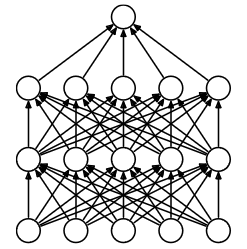
\includegraphics[scale=0.35]{src/Design/assets/before_dropout.png}}
    \subfloat[After dropout]{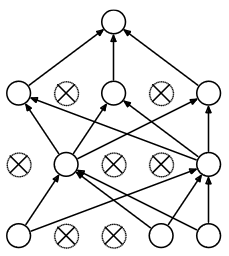
\includegraphics[scale=0.45]{src/Design/assets/after_dropout.png}}
    \end{center}
    \caption{Dropout layer}\label{dropout_layer}
\end{figure}
% The dropout layer is used in NN as a method of regularization to prevent overfiting~\cite{dropout}.
% This layer breaks connections between layers for some parts of the data. The gradients of these elements are equal to zero.
The main idea of Dropout is to randomly and temporarily exclude neurons from the network during training. At the same time, 
each neuron has the probability of being "turned off" at each iteration of network training. This forcibly makes the network 
less capable of memorizing specific patterns, which helps the network generalize its knowledge to new data.

Using Dropout usually improves the generalizing ability of the model and prevents overfitting, especially in cases where the 
training sample is small or when the model has a large number of parameters.

If usually neural network works like this:
\begin{enumerate}
    \item $\overline{z}^{(l)} = \overline{w}^{(l)}\cdot \overline{y}^{(l-1)}$
    \item $\overline{y}^{(l)} = f(\overline{z}^{(l)})$
\end{enumerate}
With the dropout layer, its behavior can be described in the following way:
\begin{enumerate}
    \item $r^{(l)} \sim Bernoulli(p)$
    \item $\tilde{y}^{(l)} = r^{(l)} \odot y^{(l)}$, where $\odot$ means element-wise multiplication
    \item $\overline{z}^{(l)} = \overline{w}^{(l)}\cdot {\tilde{y}}^{(l-1)}$
    \item $\tilde{y}^{(l)} = f(\overline{z}^{(l)})$
\end{enumerate}

\subsubsection{Optimizers}
As was written above in neural networks updating weights can be implemented in the following way:
\[W^{(n)} = W^{(n-1)} - \eta \nabla_W \mathcal{L}(W^{(n-1)}, X, y)\]
Where $W$ is the tensor with model weights, $X$ is the input tensor and $y$ is the ground truth tensor.

However, this approach has some disadvantages~\cite{sgd}:
\begin{enumerate}
    \item Convergence problem, using classical stochastic gradient descent (SGD) usually doesn't guarantee good convergence.
    \item Learning rate should be chosen wisely and updated during training.
    \item The same learning rate is applied to all weights, which can be a problem since not all weights are in the same distribution and scale.
    \item SGD can lead to a local minimum of a loss function, which sometimes can cause problems during inference.
\end{enumerate}
To solve these problems a lot of different approaches for updating weights were invented. In this project, two of them were tried and one of them was finally used.

\textbf{SGD Momentum}

SGD encounters challenges when navigating through ravines, where the terrain of gradient sharply curves in one dimension more than another, 
often found near local optima. In such cases, SGD tends to zigzag along the slopes of the ravine, making slow progress toward the local optimum. 

Momentum, however, addresses this issue by accelerating SGD in the direction of relevance while dampening oscillations. 
This is achieved by incorporating a fraction of the update tensor from the previous time step into 
the current update tensor. 
\[v^{(n)}=\gamma \cdot v^{(n-1)} + \eta \nabla_W \mathcal{L}(W^{(n-1)}, X, y)\]
\[W^{(n)} = W^{(n-1)} - v ^{(n)}\]
$\gamma \cdot v^{(n-1)}$ is called momentum. It is usually set to $0.9$~\cite{sgd}. 

In other words, parameter updates accumulate momentum, accelerating convergence where gradients coincide and reducing measurement updates with 
varying gradients. Consequently, the pulse promotes faster convergence and mitigates fluctuations.

\begin{figure}[h]
    \begin{center}
    \subfloat[SGD without monmentum]{
\includegraphics[scale=0.35]{src/Design/assets/sgd.jpg}}
    \subfloat[SGD with momentum]{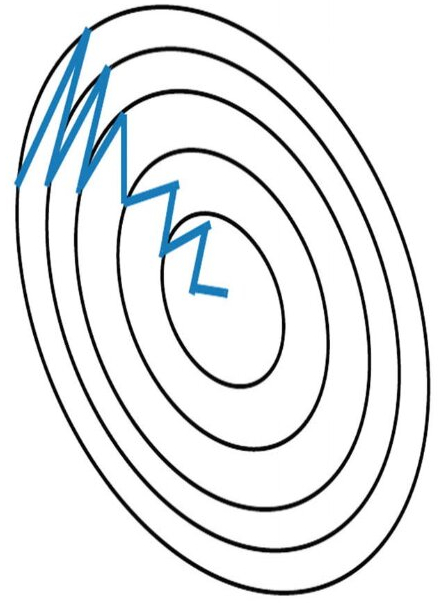
\includegraphics[scale=0.35]{src/Design/assets/sgd_momentum.jpg}}
    \end{center}
    \caption{SGD}\label{SGD}
\end{figure}

\textbf{Adam}

If SGD momentum solves the convergence problem, then Adaptive Moment Estimation (Adam)~\cite{adam} solves other problems, like learning rate scheduling, 
different learning rates for different weights and of course convergence problems. 
The algorithm of Adam can be described below:
\[g^{(n)} = \nabla_{W} \mathcal{L}(W^{(n-1)}, X, y) + \lambda \cdot W^{(n-1)}\]
\[m^{(n)} = \beta_1 \cdot m^{(n-1)} + (1-\beta_1)g^{(n)}, \text{ where } m^{(0)} = 0\]
\[v^{(n)} = \beta_2 \cdot v^{(n-1)} + (1-\beta_2){(g^{(n)})}^2 , \text{ where } v^{(n)} = 0\]
\[\widehat{m}^{(n)} = \frac{m^{(n)}}{1 - \beta_1^n}\]
\[\widehat{v}^{(n)} = \frac{v^{(n)}}{1-\beta_2^n}\]
\[W^{(n)} = W^{(n-1)} - \eta \cdot \frac{\widehat{m}^{(n)}}{\sqrt{\widehat{v}^{(n)}} + \varepsilon} \]
Here's $\eta$ is the common learning rate, $\beta_1, \beta_2$ parameters for computing running averages of gradient and its square, 
$\lambda$ is weight decay coefficient, it adds L2 regularisation for the optimizer. Authors of the algorithm suggest to use $\beta_1 = 0.9$, 
$\beta_2 = 0.999$, $\varepsilon = 10^{-8}$

The benefits of Adam are that:
\begin{enumerate}
    \item It computes adaptive learning rates for each parameter
    \item It stores bias-corrected first and second moment estimates of the exponentially decaying average of past gradients
    \item It applies L2 regularisation
\end{enumerate}

Even though Adam uses techniques of SGDM it's not obvious which optimizer is better~\cite{adam_vs_sgd}. It turns out that sometimes SGDM performs better.
That's why both optimizers were tried in the project. The choice and its reason are described in the implementation chapter.

\subsection{General project design}
As it was written in the Project planning chapter the project was divided into three big parts. The code base is shown in Figure~\ref{code_base}
\begin{figure}[h]
    \begin{center}
    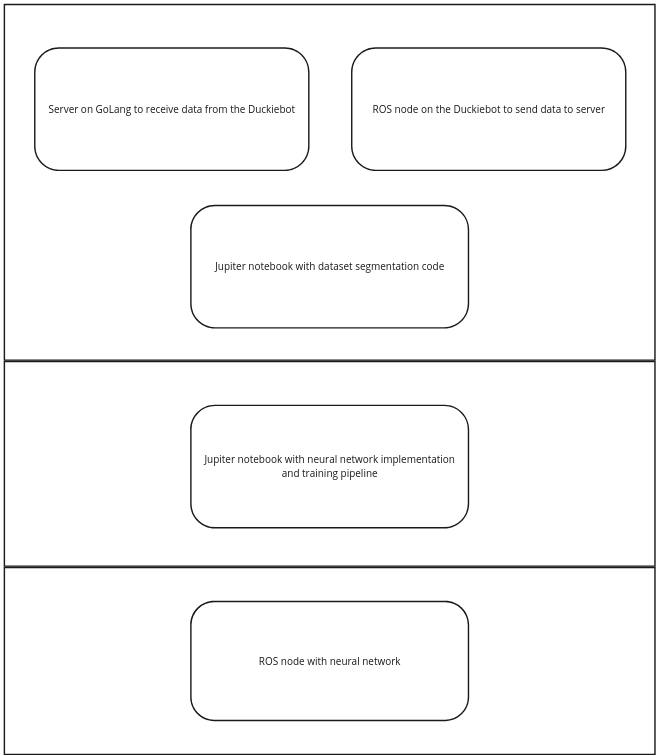
\includegraphics[scale=0.35]{src/Design/assets/code_base.png}
    \end{center}
    \caption{Code base}\label{code_base}
\end{figure}
\subsubsection{The Server}
For the server, it was decided to use a simple socket architecture. 
The server was able to handle multiple requests simultaneously, even though the Duckiebot can't asynchronously send data 
(a new photo was sent to the server only after the previous one was fully sent), writing data to disk was a bit slower than receiving pictures via WiFi. 
So a new request could come before the previous was completed. 
\subsubsection{Jupiter notebooks}
The use of Jupiter notebooks is usually in research projects. 
This technology provides the ability to execute various parts of the code without having to execute the entire pipeline. 
Since writing ML models is divided into analyzing the dataset, writing the model itself, training and testing it, 
the ability to run different parts of the code, saving variables and states after other runs is very useful.
This feature also allows you to abandon writing unit and integration tests at least at the research stage, since in case of an error, 
you can immediately see which part of the code is not working, as well as errors similar to differences in the input format are easily identified and corrected.

In addition to all the described below benefits, Jupiter notebooks are easily convertible to regular Python files, which makes migration from the research stage
to the deployment extremely easy.

\subsubsection{Deployment on the Duckeibot}
The Duckiebot is run under ROS.\@ So to deploy something on it the ROS node should be created. It was decided not to create a new ROS node, but to use the existing one,
which was used for an old lane segmentation algorithm. Moreover, the output of the created algorithm is fed into the part of the old lane segmentation algorithm.
This was done to use already existing and working code to communicate with the lane-following algorithm. However, from old algorithm part with segmentation was 
removed and only the part with converting the color mask to required for lane-following algorithm input was saved.
\section{Implementation}
\subsection{Introduction}
This chapter is also divided into 3 sections because the implementation of each step of the project has its specificity.
\subsection{Implementation of dataset collecting and segmentation}
\subsubsection{Server implemetation}
As it was described in the Design chapter, for the server it was decided to use GoLang and a simple socket server. 
The using of goroutines was almost the perfect solution for the implementation of asynchronous server~\cite{goroutines}\cite{go_shedulers}.
The technology of the goroutines is extremely efficient and perhaps, even too efficient for this server, however, in addition to the speed 
of operation, they are extremely easy to implement.

Benchmarks for the implementation of the asynchronous task approach in different programming languages are shown in table~\ref{tab:multithreading_benchmarks}.

\begin{table}[h]
    \centering 
    \begin{tabular}{|c|c|}
        \hline
        Programming language & Benchmark results in milliseconds\\ \hline
        GoLang & 22.717915 \\ \hline
        C++ & 36.1088 \\ \hline
        Rust & 75.88563631 \\  \hline
        Python & 106.35573348 \\ \hline
    \end{tabular}
    \caption{Benchmarks of multithreading in different programming languages}\label{tab:multithreading_benchmarks}
\end{table}

The server was local, so there was no need for a static IP address, however, each day it was needed to change the IP address on the client part.
\subsubsection{ROS node implementation}
For the client part, it was decided to use pure Python. Although the Duckietown project has the implementation of the MQTT bridge, 
this technology was relatively slow in comparison to pure Python on the client side and GoLang on the server. As was shown in the previous section Go implementation of 
Goroutines (as a multithreading paradigm) is one of the most efficient in terms of implementation and runtime speed. So the only task was to develop a client part. Because 
the Duckietown project uses Python as the main language for development, it was decided to create a simple HTTP client to send data to the Go server on 'pure Python'.
\subsubsection{Marking up algorithm implementation}
As it was written in the chapters above the EM algorithm was used for marking up. It was decided to use Sklearn's realization of the algorithm. 
However, the implementation wasn't so easy. Using the whole image wasn't efficient. The upper part of the image consists of a lot of different colors, 
which brings a noise to mark up. 
In order to get rid of the noise, it was decided to crop the upper half of the image. This both reduced noise and reduced the amount of data to process,
which increased the speed of markup.
Also, using the EM algorithm with only one input image per forward pass brought a lot of noise, so it was decided to combine the images into batches of 500 pieces 
(it could not be increased due to lack of RAM). The result is a relatively high-quality markup.
\subsubsection{Validation of the markup}
Validation of the result markup was carried out manually. Out of 9,000 images, 500 were discarded due to poor markup.
The rest of the images were used in neural network training.



\subsubsection{Images in the dataset}
The resulting dataset consists only of three types of images. 
\begin{enumerate}
    \item Raw cropped image. A neural network was trained on these images.
    \item The mask. It's just a pixel map that was used as a ground truth for network training. 
    \item An image containing both a raw image and a mask. This part of the dataset is necessary for validation by other people. Since the dataset was published 
    in the public domain, it can be supplemented with other images, because of this, some images can be replaced with less noisy ones. For the convenience of the 
    validation process, this part of the dataset was created.
\end{enumerate}
There is no other data in the dataset.

\subsection{Neural network implementation}
\subsubsection{Choosing hyperparameters}
The architecture of the deep learning model was described in the Design chapter, however, the process of choosing hyperparameters of the model is described here.
Using grid search for choosing hyperparameters isn't so usual in deep learning, because it consumes a lot of time and computational resources. 
The first few runs of the training step of the neural network were without a grid search. A few parameters were changed during those runs but that change didn't give
good enough results. So it was decided to use grid search for choosing hyperparameters. However because of the lack of computational resources not all combinations of 
hyperparameters were tested, but 36 combinations with the most important hyperparameters were tried. As validation metrics recall and precision were used:
\[RECALL = \frac{TP}{TP + FN}\]
\[PRECISION = \frac{TP}{TP + FP}\] 
Because these metrics can be computed only for binary classification, they were computed twice: for yellow and white pixels.
The result of the validation step of training is represented in the table~\ref{tab:validation_step}.
\begin{table}[h]
    \centering 
    \begin{tabular}{|c|c|c|c|c|c|c|c|c|}
        \hline
        Optimizer & Kernel size & Yellow weight & White weight & Validation loss & Yellow recall & White recall \\ \hline
        Adam & 3 & 5.0 & 5.0 & 0.157 & 0.764 & 0.929 \\ \hline
        Adam & 3 & 5.0 & 3.0 & 0.147 & 0.750 & 0.901 \\ \hline
        Adam & 3 & 5.0 & 2.0 & 0.170 & 0.771 & 0.734 \\ \hline
        Adam & 3 & 7.0 & 5.0 & 0.139 & 0.818 & 0.945 \\ \hline
        Adam & 3 & 7.0 & 3.0 & 0.153 & 0.809 & 0.863 \\ \hline
        Adam & 3 & 7.0 & 2.0 & 0.159 & 0.783 & 0.804 \\ \hline
        Adam & 3 & 10.0 & 5.0 & 0.140 & 0.835 & 0.955 \\ \hline
        Adam & 3 & 10.0 & 3.0 & 0.140 & 0.846 & 0.906 \\ \hline
        Adam & 3 & 10.0 & 2.0 & 0.139 & 0.854 & 0.830 \\ \hline
        Adam & 5 & 5.0 & 5.0 & 0.140 & 0.777 & 0.946 \\ \hline
        Adam & 5 & 5.0 & 3.0 & 0.149 & 0.765 & 0.890 \\ \hline
        Adam & 5 & 5.0 & 2.0 & 0.145 & 0.792 & 0.794 \\ \hline
        Adam & 5 & 7.0 & 5.0 & 0.174 & 0.803 & 0.915 \\ \hline
        Adam & 5 & 7.0 & 3.0 & 0.154 & 0.780 & 0.911 \\ \hline
        Adam & 5 & 7.0 & 2.0 & 0.165 & 0.772 & 0.745 \\ \hline
        Adam & 5 & 10.0 & 5.0 & 0.133 & 0.847 & 0.951 \\ \hline
        Adam & 5 & 10.0 & 3.0 & 0.151 & 0.821 & 0.896 \\ \hline
        Adam & 5 & 10.0 & 2.0 & 0.165 & 0.796 & 0.826 \\ \hline
        SGDM & 3 & 5.0 & 5.0 & 0.173 & 0.802 & 0.904 \\ \hline
        SGDM & 3 & 5.0 & 3.0 & 0.202 & 0.752 & 0.804 \\ \hline
        SGDM & 3 & 5.0 & 2.0 & 0.197 & 0.791 & 0.794 \\ \hline
        SGDM & 3 & 7.0 & 5.0 & 0.182 & 0.796 & 0.893 \\ \hline
        SGDM & 3 & 7.0 & 3.0 & 0.177 & 0.805 & 0.854 \\ \hline
        SGDM & 3 & 7.0 & 2.0 & 0.181 & 0.803 & 0.775 \\ \hline
        SGDM & 3 & 10.0 & 5.0 & 0.180 & 0.832 & 0.917 \\ \hline
        SGDM & 3 & 10.0 & 3.0 & 0.210 & 0.805 & 0.834 \\ \hline
        SGDM & 3 & 10.0 & 2.0 & 0.184 & 0.849 & 0.874 \\ \hline
        SGDM & 5 & 5.0 & 5.0 & 0.162 & 0.806 & 0.907 \\ \hline
        SGDM & 5 & 5.0 & 3.0 & 0.181 & 0.794 & 0.811 \\ \hline
        SGDM & 5 & 5.0 & 2.0 & 0.224 & 0.738 & 0.690 \\ \hline
        SGDM & 5 & 7.0 & 5.0 & 0.177 & 0.806 & 0.895 \\ \hline
        SGDM & 5 & 7.0 & 3.0 & 0.203 & 0.779 & 0.819 \\ \hline
        SGDM & 5 & 7.0 & 2.0 & 0.186 & 0.811 & 0.768 \\ \hline
        SGDM & 5 & 10.0 & 5.0 & 0.178 & 0.869 & 0.933 \\ \hline
        SGDM & 5 & 10.0 & 3.0 & 0.192 & 0.827 & 0.814 \\ \hline
        SGDM & 5 & 10.0 & 2.0 & 0.203 & 0.825 & 0.787 \\ \hline
    \end{tabular}
    \caption{Results of validation step with different hyperparameters}\label{tab:validation_step}
\end{table}

These results are not precise, because to be so, each set of hyperparameters should be validated a few times, however, because of the lack 
of computational resources on Google Colab these sets were validated just one time each. It took 12 hours to validate these sets and consumed almost all resources of 
Google Colab.

The weights of colors which are described in the table are weights for a cross-entropy loss function. As it's shown in the table these weights are crucial 
for the target metrics. This happens because the dataset isn't balanced in terms of color distribution. The amount of pixels with the color of the road is much more 
than any other color, also the amount of pixels of white color is more than yellow ones. That's why weights were required. 

\subsubsection{Dataset preprocessing and augmentations}

As was described in the collecting of the Dataset section for the neural network input images also cropped in the top. 
During training, the augmentations were also applied to all images to emulate the light of LEDs (images with real light of LEDs can't be marked up by the EM algorithm.
The resulting markup would be extremely noisy).
Used augmentations:
\begin{enumerate}
    \item Random brightness and contrast and random tone curve --- to emulate even more different light conditions/
    \item RGB shift and HSV shift to emulate LED light.
\end{enumerate}
\subsubsection{Libraries}
During the implementation of the neural network different libraries were used:
\begin{enumerate}
    \item PyTorch for implementation of the neural network and training pipeline
    \item Albumentation for creating augmentations
    \item TorchVision and OpenCV for preprocessing training data
    \item TorchLightning for implementation training pipeline
\end{enumerate}
Also, the Tensorboard extension for Jupiter notebooks was used for visualization changes of the target metrics during training.

\subsection{Deployment}
\subsubsection{Introduction}
During the deployment step, a lot of problems were discovered. Also single run of the algorithm on the Duckiebot consumed a lot of time to build and start the Docker
image. In this section solutions to these problems will be described as well as the general workflow of the deployment step.
\subsubsection{Choosing the Docker image}
To implement the neural network the PyTorch library with Cuda integration was required.
firstly it was decided to take a basic Cuda image and after that add an empty duckietown-core image to it. However, in the Duckietown Github, a basic Duckietown image
with included Cuda was found. So it was decided to use this image. 

However, during implementation troch2trt and TorchVision libraries were required for the image. Installing these libraries via standard pip instructions wasn't available,
so it was decided to include instructions for these installations in the Dockerfile. So finally a new base Docker image was created and published as a template image.
Also, this image is used in the project.

\subsubsection{Deploying the neural network}
To deploy the neural network on the bot two things were required:
\begin{enumerate}
    \item Import code of the neural network
    \item Import weights of the neural network
\end{enumerate}
These steps were done. 

After that, the neural network was run in test mode. It wasn't used as input for the lane-following algorithm, but it published the resulting masks into the debug 
ROS topic, they were later visualized in the special tool.
\begin{figure}[htbp]

        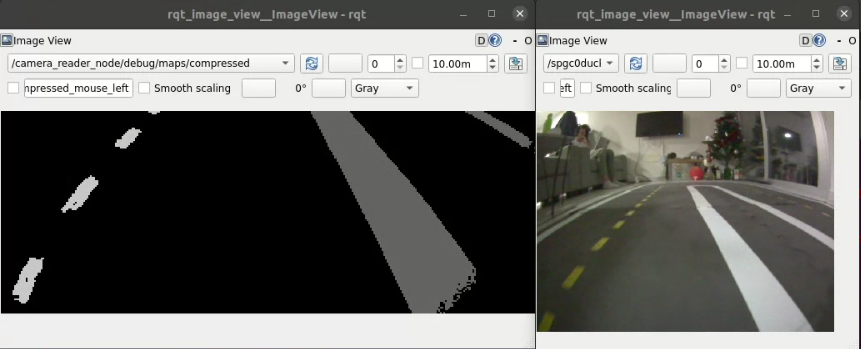
\includegraphics[scale=0.5]{src/Implementation/assets/first_run.png}
    \caption{Output of the first run}\label{fig:first_run}
\end{figure}
During this step, it was discovered that neural network has two problems:
\begin{enumerate}
    \item The whole pipeline of image processing took about 120 milliseconds.
    \item The neural network required a few iterations to speed up.
\end{enumerate}

The first problem was partly solved, but the second remained actual, so it was decided to run a few iterations of the algorithm before sending a signal that 
the Duckiebot is ready to work.

\subsubsection{Torch2trt library}
To solve the first problem described in the previous section it was decided to use the torch2trt library. This library provides an opportunity for easy conversion of  
torch tensors to TensorRT tensors. TensorRT is SDK by Nvidia for high-performance tensor computations. Jetson Nano was developed by Nvidia so there was a hope,
that using this library could increase the speed of computations. This hope was justified. Using torch2trt increased performance twice. However, Installing 
torch2trt wasn't an easy task as it was mentioned in the Docker image subsection. This library couldn't be installed via pip because of the specificity of the hardware, 
building this library from source code was also tricky because the full installation wasn't available due to outdated software in the base Duckietown docker image, 
which couldn't be updated because of backward compatibility problems. 
Luckily partial installation could be performed and this type of installation provided the required speed boost so this half-measure was left.
\subsubsection{Merging neural network and lane-following algorithm}
The merging process was a pretty difficult step. The lane-following algorithm accepts input as a list of segments. 
However, the neural network output is a pixel map of road markup. So it was decided to use the existing algorithm of road markup segmentation but without its main part.
the road markup segmentation part was removed from the existing algorithm. The pipeline is described below:
\begin{enumerate}
    \item Output of neural network is transformed into a multichannel image.
    \item This image is colored into the desired colors: black, white and yellow.
    \item The result is fed into the existing algorithm.
\end{enumerate}  
As a result, the time consumed per image increased by 20 milliseconds, but this approach significantly decreased the time for implementation. 
In addition, because this algorithm was already in use the problem of bugs was also solved. 
\subsubsection{Conclusion}
As a result, the full pipeline for one image takes about 50--70 milliseconds which is a pretty good result. This speed is more than enough for lane following algorithm 
to make decisions on the next action of the Duckiebot.
\subsection{Chapter conclusion}
As it was written in this chapter implementation of the project wasn't an easy task. However, the project was done. There was a lot of research done and a lot of 
code was written, but most of this code was just a utility. The algorithm itself is really small in terms of code volume, however, there was a lot of code behind it, which was
required to write this small amount. 
\section{Testing}
\subsection{Introduction}
The main goal of this project was to develop an algorithm for autonomous marking up of a dataset and create an algorithm for the detection of road markup based
on deep learning algorithms. The specifics of the project imply a special approach to code testing, which will be discussed in this chapter. It is important to 
notice that all parts of the project that are not machine learning algorithms were auxiliary and were run strictly under the supervision of the developer, which
makes testing of these parts of the project not optional, but at least questionable.

\subsection{Functional testing}
\subsubsection{Machine learning algorithms automated testing}

Testing is included in the mandatory pipeline for creating a machine-learning algorithm. The selection of hyperparameters described in the chapter above, 
as well as the choice of the model architecture is based on the results of running the model on a separate part of the dataset, which was not used in training. 
This part is called the test part.

This approach allows one to achieve several goals at once:
\begin{enumerate}
    \item Check the performance of the algorithm, i.e.\ whether it falls on different data.
    \item Check the compliance of the algorithm with the specified requirements for the format of input and output data
    \item Check the correctness of the algorithms, i.e.\ how well it copes with the task.
\end{enumerate} 
If the first two points are checked quite easily (if the neural network does not meet the input/output requirements or crashes on some data, then the algorithm will 
fail during the run of the test sample). The third point presupposes more complex reasoning. Since machine learning algorithms almost never give
a truly correct answer, it is impossible to test such algorithms only for matching the correct answers. For machine learning algorithms, it is normal sometimes 
to give incorrect answers, however, the purpose of training such algorithms is to minimize error cases. Based on this, hyperparameters and architecture are selected. 

Therefore, it can be said that automated functional testing is embedded in the process of developing machine-learning algorithms and does not require additional code 
in the form of unit tests.

\textbf{EM algorithm}

For the EM algorithm, things get even more complicated. Since there are no correct answers in the training sample, checking the correctness of the algorithm was impossible in
automatical mode. Moreover, checks based on expecting the same output for the same input, can't be performed too. Since the initialization of hidden class labels in 
the EM algorithm occurs randomly, this algorithm may give slightly different answers to the same input data and this cannot be called
an incorrect behavior of the algorithm.

\textbf{Neural networks layers unit testing}

For neural networks, it is possible to write unit and integration tests when they are developed from scratch. That is, all the mathematics described in the chapters 
above is written by the developer himself. However, this project used the PyTorch library, which provides already-written layers of neural networks. 
Therefore, unit testing of these blocks is unnecessary.

\textbf{Deliberately incorrect data}

The only objective reason for creating functional tests for machine learning algorithms is to check the performance of algorithms with deliberately
incorrect data. However, these tests were not written in this project for the following reasons:
\begin{enumerate}
    \item The neural network is published within the Duckietown repository, the only possible input of this algorithm is a three-channel image of 480*640 pixels. 
    Therefore, checking the input data for compliance with the specified data type is unnecessary. If the algorithm is taken from the repository and used for other 
    purposes, I am not responsible for this in accordance with the MIT license.
    \item The neural network is written exclusively for recognizing road markup. If the camera of the Dackiebot is directed at something else, the neural network will not 
    fall but will give an unpredictable result. Checking for the presence of a road in the frame could be integrated into the algorithm, however, this would increase 
    the time cost of processing a single frame. And since Duckiebot is supposed to be used only on a landfill simulating a road, frames with such content can be obtained 
    either as inappropriate using Duckiebot, which is not my area of responsibility, or as a result of an error that causes the bot to leave the landfill, but such cases
    are exceptional and must be controlled by a human, which is why it was considered checking for the presence of a road to be an unnecessary complication of the algorithm, 
    which will lead to a deterioration in operating time.
\end{enumerate}

\subsubsection{Non-machine learning algorithms automated testing}
As it was written in the Introduction subsection all non-machine learning algorithms and applications were written only for inner use. Moreover, they were used
only under developer control, so writing functional tests for this part of the project was unnecessary.

However, one non-machine learning part was released. It was a ROS node with an implemented neural network in it. 
But this node mostly consists of code of the old algorithm, so bugs can be only in machine learning part, but as it was written above, 
the neural network was tested during the training phase so once again the creation
of any automated functional tests was redundant. 

\subsubsection{Manual functional testing}
As it was written above it was decided to get rid of using an automated testing approach. However, leaving the project completely untested would be a terrible mistake.
As a test, it was decided to do a very simple thing. Start the autopilot and look at its behavior. 

As a result of this approach, minor errors were identified, which were immediately corrected. However, more significant problems with the bot have been found.
The bot drove out of the lane in turns and also interpreted the white floor as part of the road markings, which sometimes led to unpredictable behavior.
These errors are described in more detail in the chapter below and they will not be considered here.

\subsection{Non-functional testing}

\subsubsection{Introduction}
In fact, non-functional testing has been discussed throughout this document. Since the speed of the algorithm is a key
aspect of its development. Then the speed of the algorithm was measured many times in different conditions.

\subsubsection{Speed of the algorithm}

The speed of the neural network was checked at the time of its creation, in Google Colab, as well as directly on Duckiebot. Based on this data, decisions were made
to use the torch2trt library to reduce the execution time of the data processing pipeline.

Also, according to the results of the benchmarks, an interesting observation was made, despite the shared GPU and CPU memory, the torch library takes time to send data
to the GPU memory, which looks strange. This observation paved the way for further research and development of a driver for the bot's camera so that the resulting 
image was immediately in PyTorch-GPU-tensor format. This does not apply to the current project, but the implementation of such a driver in theory will be able 
to speed up the algorithm's operation time by at least 3 times.

\subsection{User testing}
Since the project was a research project, it does not involve an end user. Therefore, no user testing was carried out.

\subsection{Summary}

\noindent At the end of the chapter, it should be noted that the testing in the project was carried out, although not in a completely ordinary execution.

\noindent  In the project, it was decided to abandon unit and integration testing due to the redundancy of these tests, as well as the time to write them. 
The neural network was tested during its training, the EM algorithm was tested during its operation, as it was launched under the supervision of the developer.
Checking the compatibility of the algorithm with the software was carried out in real conditions, since this approach, on the one hand, does not require time to write
testing code, and on the other hand, makes it possible to fully assess the performance of the project.

\noindent Benchmarks of the operating time of the neural network, the neural network pipeline and the entire data processing pipeline were also carried out. 
Based on these data, it was decided to use additional libraries to speed up the algorithm. The benchmark results not only helped to improve the project but also 
laid the foundation for future developments in Duckietown.

\noindent User testing was not performed due to the absence of an end user.

\noindent The results of the testing phase were studied and taken into account during the development of the project.
\section{Evaluation, Conclusions and Future Work}
\subsection{Project Objectives}
As a result of the project, a few things were made:
\begin{enumerate}
    \item Collected, marked up and published dataset
    \item Created deep learning algorithm for road markup detection
    \item The algorithm was deployed on Duckiebot
\end{enumerate}

The dataset is available on my GitHub repository it is also been published in the official Duckietown Slack. 

The model is also available on my GitHub with the Docker image for Duckiebot

\subsection{Self-Evaluation}
During this project, I've learned a lot about computer vision, docker, ROS and the Duckietown project. I also learned how to collect and publish a good dataset.

On the other hand, I've figured out some of my weaknesses. Doing paperwork is pretty hard for me. So this skill should be developed.

\subsection{Project Evaluation}
Overall the main goal was achieved. The road markup segmentation algorithm works almost as well as I wanted at the start. 
It is light-insensitive, doesn't change its behavior with different colors of the Duckiebot's LEDs and takes only 1 millisecond to process one image.
However there are a few problems that are not connected to the algorithm itself, but affect the Duckiebot behavior, 
making an evaluation of the project not so obvious.
\begin{enumerate}
    \item Transfering data from/to GPU memory is the first problem. The Duckiebot is powered by Jetson Nano by Nvidia. It has shared GPU and CPU RAM, but 
    existing libraries and drivers available for Duckiebot do not allow it to take advantage of this. That is why transferring to and from GPU RAM takes 
    the most time in the pipeline. To solve this problem I have to rewrite the driver which is obviously beyond the scope of the project
    \item The current lane-following algorithm and servo motors are the second problem. To make the algorithm fast and precise I cut off the upper half of the input 
    image. However, when I pass the output of my algorithm to the lane following algorithm the Duckiebot sometimes behaves weirdly. 
    This is especially noticeable on the turns of the road. To perform a turn the Duckiebot drives out of its lane, but comes back soon after the turn. 
    The reason for this behavior is that lane following algorithm treats 
    This algorithm is part of the base docker image of the Duckiebot, so I can't change it. And servo motors are obviously beyond the scope of the project 
    and the Computing University course
    \item The last problem is the white floor. My algorithm usually treats the white floor as the white line of the road markup. It is not a big problem of 
    the algorithm, but to correctly evaluate the project it is better to use rooms with dark floors for a testing polygon or enlarge a polygon with empty black tiles 
    on the edges. 
In addition the neural network was tested in a few configurations. You can find the results in table~\ref{tab:p_results}. All this runs were pretty good in terms of accuracy, 
but had a difference in images per second. It was decided to use the second configuration for the resulting approach, as it's pretty accurate, but in the same time 
not so heavy in computartional time.

\begin{table}[h]
    \centering 
    \begin{tabular}{|p{1.7cm}|p{2.3cm}|p{5.2cm}|p{5.2cm}|p{1.7cm}|}
        \hline
        Image size & NN initialisation time & First run time (average time for full NN pipeline with transfering data to and out of GPU memmory)& Average time per image (average time for full NN pipeline with transfering data to and out of GPU memmory)& Accuracy (percent of time spent, when bot was on right position)  \\ \hline
        $640 \times 120$ &  123 seconds & 320 milliseconds (3332 milliseconds) & 1.3 milliseconds (113 milliseconds) & $90\%$ \\ \hline
        $320 \times 60$ &  107 seconds & 9 milliseconds (672 milliseconds) & 1 millisecond (67 milliseconds)& $83\%$\\ \hline
        $160 \times 30$ &  58 seconds & 6.5 milliseconds (514 milliseconds) & 1 millisecond (43 milliseconds)& $80\%$\\ \hline
    \end{tabular}
    \caption{Project results}\label{tab:p_results}
\end{table}

\end{enumerate}
\begin{figure}[htbp]
    \centering
    \subfloat[Raw image of the road with floor]{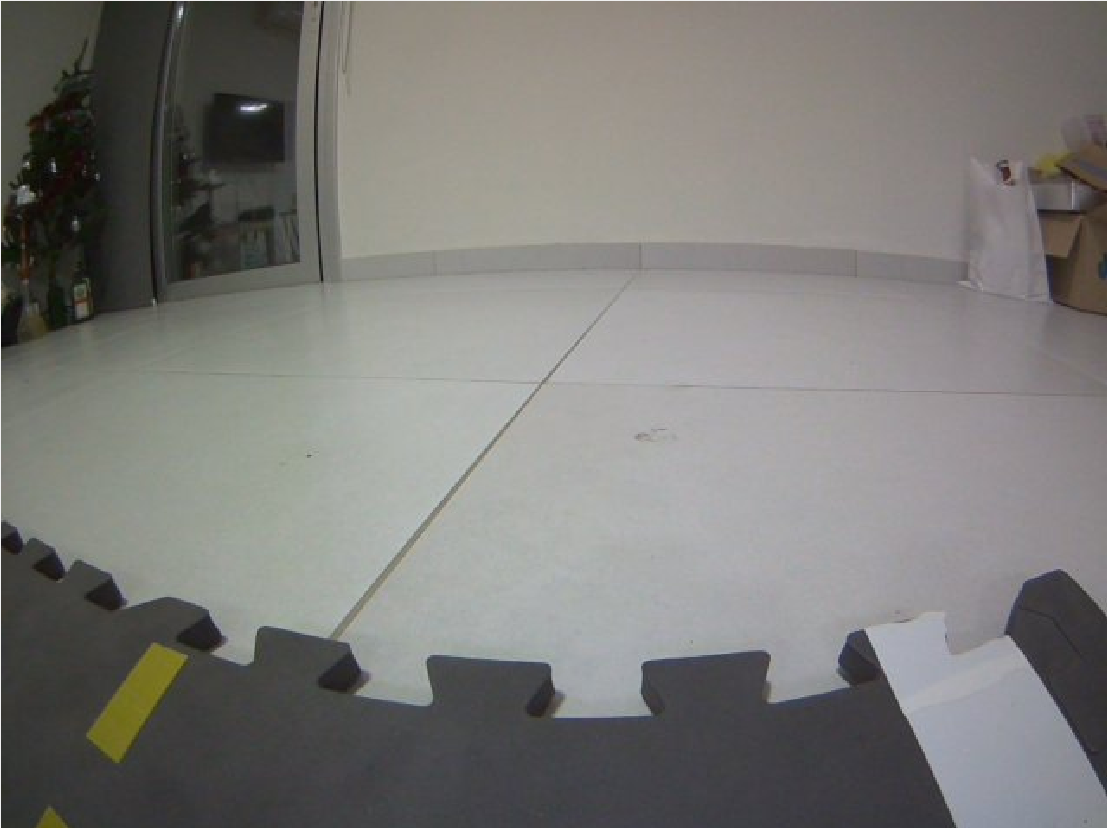
\includegraphics[scale=0.1]{src/EvaluationConclusionsAndFutureWork/assets/masks02.png}}
    \subfloat[Mask of the road with floor]{
\includegraphics[scale=0.1]{src/EvaluationConclusionsAndFutureWork/assets/masks01.png}}
    \\
    \subfloat[Raw image of the road without floor]{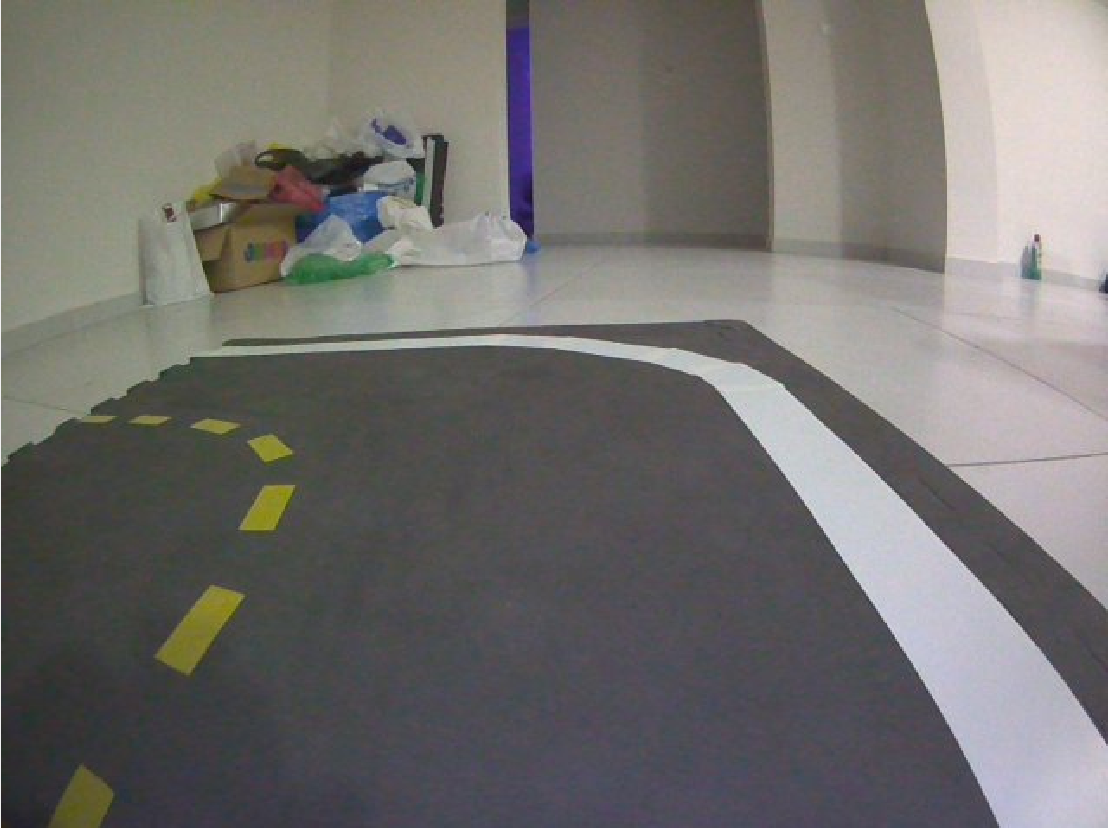
\includegraphics[scale=0.1]{src/EvaluationConclusionsAndFutureWork/assets/mask3.png}}
    \subfloat[Mask of the road without floor]{
\includegraphics[scale=0.1]{src/EvaluationConclusionsAndFutureWork/assets/mask4.png}}
    \caption{Masks for different parts of the road}\label{fig:masks}
\end{figure}
\subsection{Applicability of Findings to the Commercial World}
This project is a research project, so it can't be directly applied in the commercial world. However, I've managed to create a good algorithm and collect a
pretty huge and well-marked dataset, which can help in developing the Duckietown project. Also, my contribution can help me find a job in computer vision, 
especially in self-driving car fields. 
\subsection{Conclusion}
As a result of the project the dataset was collected, marked up and published and the algorithm was created, deployed and published.
I've learned a few new things, like working with Docker or creating soft for robots. This project inspired me to dive into the world of reinforcement learning
to be able to create not only computer vision algorithms but also algorithms like autonomous lane following. The project was interesting and complicated, 
sometimes boring. But overall when Duckiebot finally drove by itself I was extremely happy.
\subsection{Future work}
Because of a lack of money for creating the polygon, I've decided to get rid of the red lines, which mark the beginning of the road intersection zone. So as future 
work adding a red line to the dataset can be considered. Also, these things can be done (and I'll probably do it, but not in the scope of this project):
\begin{enumerate}
    \item Combining my algorithm with the object detection algorithm. This step will fully close the lane-following problem because Duckiebot will be able to
    drive in the traffic lane, but also be able to detect objects (like duckies, which imitate pedestrians).
    \item Creating algorithm based on photogrammetry for crossing road intersection. This step in combination with the first one will fully solve the self-driving problem, 
    as the bot will be able to drive on any type of city road: basic road and traffic intersections.
    \item Improving lane following algorithm in the base image of Duckiebot.
    \item Create a driver for the Duckiebot camera so that it receives images immediately in the PyTorch-GPU-tensor format, so as not to waste time converting the tensor
    from CPU-tensor format to GPU-tensor. This driver can greatly speed up the work of computer vision algorithms on bots.
\end{enumerate}


\bibliographystyle{apalike} % We choose the "plain" reference style
\bibliography{refs} % Entries are in the refs.bib file
\newpage
\appendix
\section{Appendix 1}
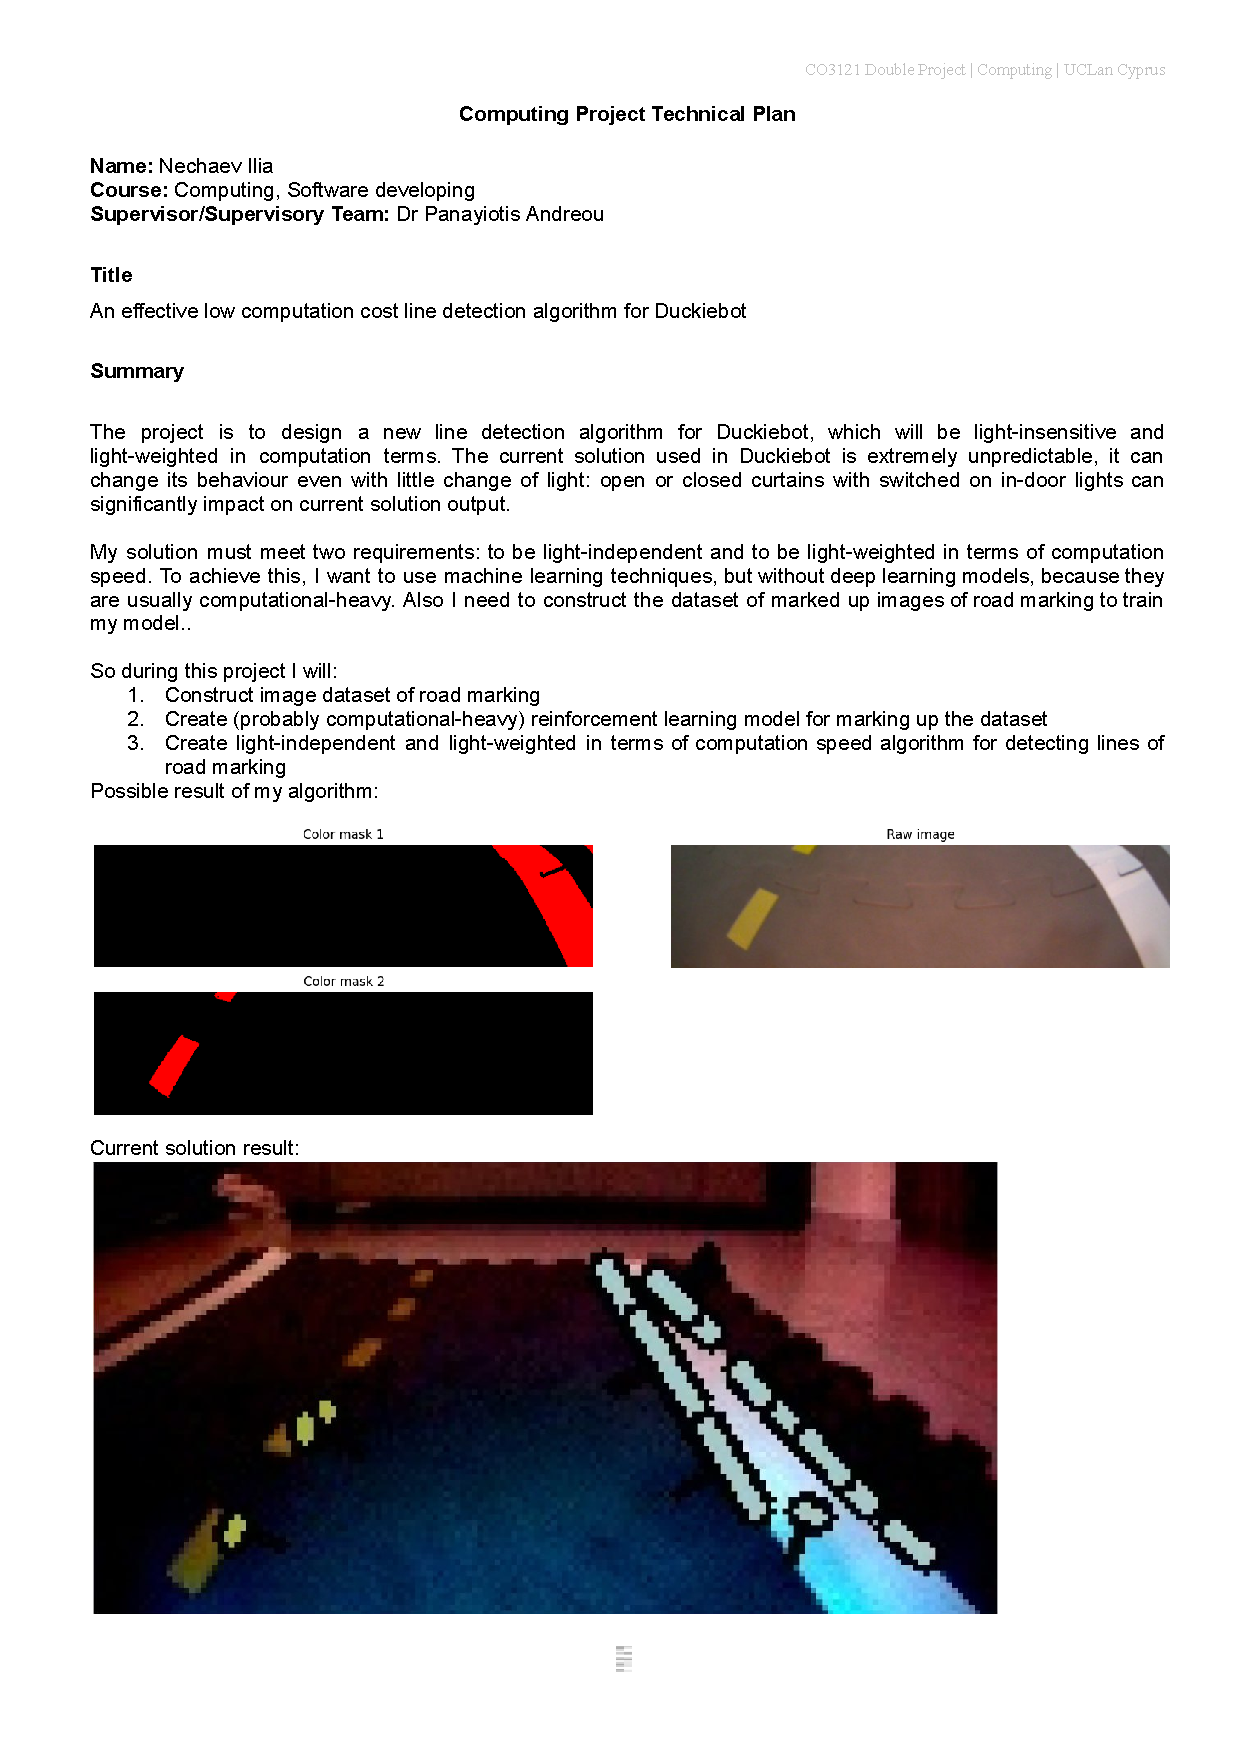
\includepdf[pages=-]{plan.pdf} % Title page

\end{document}